\documentclass[lettersize,journal]{IEEEtran}

\usepackage{amsmath,amssymb,amsfonts}
\usepackage{amsthm}
\usepackage{mathrsfs}
\usepackage{mathtools}
\usepackage{bm}
\usepackage{xcolor}
\usepackage{graphicx}
\usepackage{tikz}
\usetikzlibrary{positioning,fit,backgrounds,arrows.meta}
% Colors for the inlined pipeline overview diagram (Fig.~\ref{fig:overview}).
\definecolor{snunavy}{HTML}{1F4E79}
\definecolor{snunavy2}{HTML}{2F6690}
\definecolor{snulight}{HTML}{EAF2F8}
\definecolor{snulight2}{HTML}{F4F8FB}
\definecolor{accentred2}{HTML}{B94A48}
\definecolor{accentredlight}{HTML}{FBEAEA}
\definecolor{textgray}{HTML}{444444}
\usepackage{algorithm}
\usepackage{algorithmic}
\usepackage{cite}
\usepackage[colorlinks=true,allcolors=blue]{hyperref}

\usepackage{accents}
\newcommand{\ubar}[1]{\underaccent{\bar}{#1}}

% Extra vertical breathing room between stacked double-column floats (Tables I--III).
\setlength{\dblfloatsep}{18pt plus 2pt minus 2pt}
\setlength{\dbltextfloatsep}{22pt plus 2pt minus 4pt}

\DeclareMathOperator*{\argmax}{arg\,max}
\DeclareMathOperator*{\argmin}{arg\,min}

\newtheorem{theorem}{Theorem}
\newtheorem{proposition}{Proposition}
\newtheorem{definition}{Definition}
\newtheorem{assumption}{Assumption}
\newtheorem{lemma}{Lemma}
\newtheorem{problem}{Problem}
\newtheorem{remark}{Remark}
\newtheorem{example}{Example}
\newtheorem{corollary}{Corollary}
\newtheorem{property}{Property}

\begin{document}

\title{Planning Meets Functional Calibration: Function Conformal Prediction for Safe Motion Planning in Uncertain Environments}

\author{First~A.~Author,~\IEEEmembership{Student Member,~IEEE},
        Second~B.~Author,~and~Third~C.~Author,~\IEEEmembership{Member,~IEEE}%
\thanks{Manuscript received Month~DD, 2026; revised Month~DD, 2026.}%
\thanks{The authors are with the Department of XXX, University XXX, City, Country
(e-mail: author@example.edu).}}

\markboth{IEEE Transactions on Robotics,~Vol.~XX, No.~X, Month~2026}%
{Author \MakeLowercase{\textit{et al.}}: Planning Meets Functional Calibration}

\maketitle

\begin{abstract}
Safe motion planning in dynamic environments requires reasoning about the
uncertainty of predicted obstacle motion without sacrificing real-time
performance. We introduce a functional conformal prediction (FCP) framework that
calibrates a high-confidence lower bound of the predicted signed distance field
(SDF) at the level of the spatial \emph{field} rather than at individual points or
trajectories. The residual SDF is represented in a data-driven functional basis
via functional principal component analysis, and a Gaussian-mixture inductive
conformal procedure yields a distribution-free upper envelope of the calibration
error. A key feature is an offline--online decomposition in coefficient space: an
accurate envelope is fitted offline, while online it is refined by a lightweight
adaptive functional conformal (AFCP) update acting only on a low-dimensional
coefficient vector. We embed the conformalized lower-bound SDF as a tightened
safety constraint in a sampling-based model predictive controller and establish
asymptotic closed-loop safety, both under exchangeability and, via the online
adaptation, under distribution shift. Experiments on the ETH--UCY pedestrian
benchmarks and a dense 3D quadrotor navigation task with hundreds of dynamic
obstacles show that FCP-MPC attains a favorable balance of safety, feasibility,
and efficiency, while keeping per-step computation far below online
uncertainty-reasoning baselines.
\end{abstract}

\begin{IEEEkeywords}
Conformal prediction, motion planning, model predictive control, collision
avoidance, signed distance fields, uncertainty quantification, safe navigation.
\end{IEEEkeywords}

\section{Introduction}
% motivation
efficient motion planning in uncertain environments with safety \& efficiency guarantees


% related works; to to be classified according to our contribution
conformal prediction for safe motion planning~\cite{lindemann2023safeplanning, dixit2023adaptive,lekeufack2024decision,mei2025perceive,shin2025egocentric,contreras2025safe,sundarsingh2026safe}



% what makes functional CP beneficial in motion planning?
\begin{itemize}
    \item representation perspective (environmental geometries often admit low-dimensional representations)

    \item recent worst-case definition of score functions for motion planning are intractable, thus requiring severe approximation in practice, e.g.~\cite{mei2025perceive,sundarsingh2026safe}.
\end{itemize}

\subsection{Notation}
For $f, g \in L^2(\mathcal{X}, d\mathbf{x})$, we denote their inner product by $\langle f, g \rangle = \int_{\mathcal{X}} f(\mathbf{x})g(\mathbf{x}) d\mathbf{x}$.



\section{Related Works}
% risk-aware motion planning

% conformal prediction for reachability


\begin{itemize}
    \item robust control: DRO~\cite{long2026sensor}

    \item navigation in dynamic environments
    \begin{itemize}
        \item perception (localization, mapping, detection, tracking, $\cdots$) \& prediction in dynamic environments
        \begin{itemize}
            \item SLAM $+$ MOT~\cite{wang2007simultaneous,coue2006bayesian}

            \item particle-based~\cite{danescu2011modeling,tanzmeister2014grid}
            
            \item random finite sets~\cite{nuss2018random,chen2023continuous}; based on~\cite{mahler2007statistical}

            \item SDF learning~\cite{park2019deepsdf,ortiz2022isdf}; mostly in 3d; may be irrelevant to ours
        \end{itemize}
    \end{itemize}

    
\end{itemize}


\section{Preliminaries}
\label{sec:preliminaries}

Our calibration machinery builds on conformal prediction (CP), a distribution-free
framework that turns a heuristic uncertainty score into sets with finite-sample
coverage. We recall the two ingredients we rely on; the functional extension
specific to signed-distance fields is developed in
Section~\ref{sec:functional_projection}.

\paragraph{Split conformal prediction.}
Given exchangeable samples $\{z_n\}_{n=1}^N$ and a nonconformity score
$s(\cdot)\in\mathbb{R}$ (larger meaning a worse fit), fix a target miscoverage
level $\alpha\in(0,1)$ and set
$\hat q = \mathsf{Quantile}_{1-\alpha}\bigl(\{s(z_n)\}_{n=1}^N\cup\{+\infty\}\bigr)$.
For a fresh exchangeable sample $z_{N+1}$,
\begin{equation}
\mathbb{P}\bigl[s(z_{N+1})\le \hat q\bigr]\ge 1-\alpha,
\label{eq:split_cp}
\end{equation}
with no assumption on the data distribution beyond exchangeability~\cite{lei2015conformal}.
We use this offline to obtain a high-confidence upper bound on the
signed-distance prediction error.

\paragraph{Adaptive conformal inference.}
When the stream is non-exchangeable (e.g.\ under distribution shift), the marginal
guarantee~\eqref{eq:split_cp} may fail. Adaptive conformal inference
(ACI)~\cite{gibbs2021adaptiveconformalinferencedistribution} instead enforces a
\emph{long-run} guarantee by updating the threshold online from the observed
miscoverage: with step size $\gamma>0$ and
$\mathrm{err}_t=\mathbb{I}[\,s_t> \hat q_t\,]$,
\begin{equation}
\hat q_{t+1}=\hat q_t+\gamma\,(\mathrm{err}_t-\alpha),
\label{eq:aci}
\end{equation}
which drives the empirical miscoverage $\tfrac1T\sum_{t}\mathrm{err}_t$ to $\alpha$
for an arbitrary, even adversarial, sequence. Our online envelope
update~\eqref{eq:acp_update} is a coefficient-space, functional instance
of~\eqref{eq:aci}, and underlies the robust safety guarantee of
Theorem~\ref{thm:asymptotic_safety_afcp}.


\section{Problem Formulation}




Let $\mathcal{Q}$ be the configuration space of a robot, and  $\mathbf{x} = \mathbf{x}(\mathbf{q}) \in \mathcal{X} \subseteq \mathbb{R}^d$ the position in the world corresponding to $\mathbf{q}\in \mathcal{Q}$ (i.e., the forward kinematics of the robot), where $d = 2$ or $d=3$.
We also use the notation $\mathcal{A} = \mathcal{A}(\mathbf{q}) \subseteq \mathcal{X}$ to denote the footprint of the robot (which is a closed subset of $\mathcal{X}$) whose configuration is $\mathbf{q}$. Defining a control input as $\mathbf{u} \in \mathcal{U}$, the dynamics of the robot is given as the equation
\begin{equation*}
\mathbf{q}_{t+1} = f(\mathbf{q}_{t}, \mathbf{u}_{t}), \quad t = 0, 1, \ldots.
\end{equation*}
We specifically consider a \emph{dynamic} environment where $t =0, \ldots, T$ is the time window and $\mathcal{O}_t \subseteq \mathcal{X}$ is the union of \emph{dynamic} obstacles at $t$ (which is often represented as an occupancy map in practice), which is \emph{completely unknown}. $\{ \mathcal{O}_t\}_{t = 0}^T$ is modeled as a set-valued random process, where the randomness of the process embraces \emph{environmental variations}. It is also assumed that each $\mathcal{O}_t$ is indepdent of $\mathbf{q}_0, \mathbf{u}_0, \ldots, \mathbf{q}_t$, which indicates that the motion of the robot does not affect the environmental occupancy $\mathcal{O}_t$.\footnote{Extending this to consider bidirectional interactions among the robot and dynamic agents is left as a future work.} We also write $\mathcal{A}_t \coloneqq \mathcal{A}(\mathbf{q}_t)$.
Finally, to model a limited perception range, we follow the formulation of~\cite{janson2018safe} and introduce a perception map $P : \mathcal{X} \times \mathscr{C}(\mathcal{X}) \to \mathscr{M}_{\text{partial}}(\mathcal{X})$, where $\mathscr{C}(\mathcal{X})$ is the collection of all closed subsets of $\mathcal{X}$ (each $\mathcal{C} \in \mathscr{C}(\mathcal{X})$ being a union of obstacles, i.e.\ the \emph{unknown} occupancy of the world), and $\mathscr{M}_{\text{partial}}(\mathcal{X})$ is the set of all measurable \emph{partial} functions on $\mathcal{X}$,
\begin{equation*}
\mathscr{M}_{\text{partial}}(\mathcal{X}) \coloneqq \bigl\{ D : \mathcal{Y} \to \mathbb{R} \;\big|\; \mathcal{Y}\subseteq\mathcal{X},\ D\ \text{measurable} \bigr\}.
\end{equation*}
Intuitively, $P(x, \mathcal{C})$ is the signed distance field (SDF) sensed from configuration $x$ when the true geometry is $\mathcal{C}$; in practice it is realized as a truncated SDF~\cite{newcombe2011kinectfusion}, which we prefer to a binary occupancy map for its smooth, distance-aware structure. The use of \emph{partial} functions accounts for the finite sensing range.
Let $\mathcal{C}_t$, $t \geq 0$, denote the time-varying occupancy, whose dynamics reflect the motion of the environment. At time $t$ the robot at $x_t = x(q_t)$ receives the observation $\widehat{D}_t = P(x_t, \mathcal{C}_t)$ with domain $\mathcal{D}_t$, and the region sensed up to time $t$ is
\begin{equation*}
\mathcal{D}_{\leq t} \coloneqq \bigcup_{\tau \leq t}\mathcal{D}_{\tau}.
\end{equation*}
On $\mathcal{D}_{\leq t}$ the observations are fused into an SDF estimate $D_{\leq t}: \mathcal{X} \to \mathbb{R}$, which is set to $0$ on the unexplored region $\mathcal{X} \setminus \mathcal{D}_{\leq t}$.
Given $\mathcal{O}_t$, We define the \emph{distance function $D_t$ associated with $\mathcal{O}_t$} as
\begin{equation*}
D_t(\mathbf{x}) \coloneqq D(\mathbf{x}, \mathcal{O}_t) = \inf_{\mathbf{x'}\in \mathcal{O}_t} \Vert \mathbf{x} - \mathbf{x}' \Vert, \quad \mathbf{x} \in \mathcal{X}.
\end{equation*}


Since the future occupancy $\mathcal{O}_{t+i}$ for $i > 0$ is unobservable at time $t$, it must be estimated from historical and contextual data, as modern prediction models do. We denote the $i$-step-ahead prediction made at $t$ by $\mathcal{O}_{t+i|t}$.
For safe motion planning, we are interested in correctly estimating the (signed) distance function at $t+i$:
\begin{equation*}
D_{t+i}(x) \coloneqq d(x, \mathcal{O}_{t+i}), \quad x \in \mathcal{X}
\end{equation*}
and its $i$-step ahead prediction be:
\begin{equation*}
D_{t+i|t}(x) \coloneqq d(x, \mathcal{O}_{t+i|t}), \quad x \in \mathcal{X}
\end{equation*}


We are primarily interested in solving the following problem:
\begin{problem}[Motion Planning with Probabilistic Safety Guarantee]\label{problem:general-motion-planning}
% Given a goal configuration and the fused SDF estimate $D_{\leq t}$, the objective is to
% generate a control policy that drives the robot toward the goal while satisfying, over
% the planning horizon $i = 1,\dots,H$,
Design a policy $\pi$ {\color{teal}(inputs \& ouputs; inputs: partial observations / outputs: $\mathbf{u}_t$)} that solves
\begin{align}\label{eq:path-collision-constraint-general}
\min_{\pi}&\quad  \sum_{t=0}^{T-1} \ell(\mathbf{q}_t, \mathbf{u}_t) + \ell(\mathbf{q}_T) \nonumber \\
\text{s.t.}&\quad \mathbf{q}_{t+1} = f(\mathbf{q}_t, \mathbf{u}_t), \quad 0 \leq t < T, \nonumber \\
&\quad \mathbb{P}\left[ \mathcal{A}_t\cap \mathcal{O}_t = \varnothing \;\text{for all}\; 1\leq t \leq T \right] \geq  1 - \alpha.
\end{align}

% \begin{align*}
% \mathbb{P}\!\left[\, D_{t+i}\!\left(x_{t+i}\right) \ge 0, \ \ \forall i \in \{1,\dots,H\} \,\right] \;\ge\; 1-\alpha,
% \end{align*}
% where $x_{t+i}$ denotes the robot position at time $t+i$ under the policy.
\end{problem}
The condition $\mathcal{A}(t) \cap \mathcal{O}(t) = \varnothing$ may be strengthened into
\begin{equation}\label{eq:collision-constraint-general}
\inf_{\mathbf{x} \in \mathcal{A}_t} D(\mathbf{x}, \mathcal{O}_t) > \delta
\end{equation}
where $\delta > 0$ is a user-specified margin between $\mathcal{A}_t$ and $\mathcal{O}_t$.
Since $\mathcal{O}_t$ is generally non-convex, the exact verification of this condition is intractable even when $\mathcal{A}_t$ is a convex polytope {\color{teal}(citation?)}. Therefore, a typical remedy for this is to approximate $\mathcal{O}_t$ or the free space $\mathcal{X} \setminus \mathcal{O}_t$ by a union of convex obstacles~\cite{zhang2020optimization,deits2015computing}. Instead of inheriting this assumption, we simply assume that $\mathcal{A}(\mathbf{q})$ is circular:
\begin{equation*}
\mathcal{A}(\mathbf{q}) = \{\mathbf{x}' \in \mathcal{X}: \left\Vert \mathbf{x}' - \mathbf{x}(\mathbf{q}) \right\Vert \leq r_{\text{robot}}  \},
\end{equation*}
in which case the constraint~\eqref{eq:collision-constraint-general} can be simplified into
\begin{equation}\label{eq:collision-constraint}
D(\mathbf{x}_t, \mathcal{O}_t) \geq \delta + r_{\text{robot}}.
\end{equation}
This can be simply checked by querying the distance function $D(\cdot, \mathcal{O}_t)$ once at $\mathbf{x}_t$. The condition~\eqref{eq:path-collision-constraint-general} is now translated into
\begin{equation}\label{eq:path-collision-constraint}
\mathbb{P}\left[ D(\mathbf{x}_t, \mathcal{O}_t) \geq \delta + r_{\text{robot}}\; \text{for all}\; 1\leq t \leq T \right] \geq 1 - \alpha.
\end{equation}
To solve Problem~\ref{problem:general-motion-planning}, the policy $\pi$ should incorporate information  collected up to $t$: $\mathcal{H}_t \coloneqq(\mathcal{O}_0, \ldots, \mathcal{O}_t)$ to obtain future safety while maintaining overall deployment efficiency.
A feasible approach that enables this is to define $\pi(\mathcal{H}_t)$ to be the solution of the following MPC problem:
\begin{align}
\min_{\substack{\mathbf{q}_{0:N}\in \mathcal{Q}\\ \mathbf{u}_{0:N-1}\in \mathcal{U}}}&\ \ \sum_{i=0}^{N-1} \ell(\mathbf{q}_{t+i|t}, \mathbf{u}_{t+i|t}, \mathbf{x}^{\text{ref}}_{t+i|t}) + \ell(\mathbf{q}_{t+N|t}, \mathbf{x}^{\text{ref}}_{t+N|t}) \nonumber \\
\text{s.t.}
&\ \ \mathbf{q}_{t|t} = \mathbf{q}_t, \nonumber \\
&\ \ \mathbf{q}_{t+i+1|t} = f(\mathbf{q}_{t+i|t}, \mathbf{u}_{t+i|t}), \quad 0 \leq i < N, \nonumber\\
&\ \ D(\mathbf{x}_{t+i|t}, \mathcal{O}_{t+i|t}) \geq \delta + r_{\text{robot}}, \quad 1\leq t \leq T. \label{eq:mpc-constraint-naive}
\end{align}
where $(\mathbf{x}_{t+1|t}, \ldots,\mathbf{x}_{t+N|t})$ is a planned path in $\mathcal{X}$ at $t$ based on $\mathbf{x}_t$ and $\mathcal{H}_t$, and  $(\mathcal{O}_{t+1|t}, \ldots, \mathcal{O}_{t+N|t})$ are \emph{predicted} occupancies at $t+1, \ldots, t+N$ from $\mathcal{H}_t$. In this paper, we adopt \emph{frontier method}~\cite{yamauchi1998frontier} that pursues both information gathering and efficiency.
On the prediction side, several different approaches are available. One common and mature approach is to estimate the kinematic states of dynamic agents through
detection and tracking dynamic agents from $\mathcal{H}_t$, then deploy motion prediction models to predict their future motions, which can be back-projected into $\mathcal{X}$ to infer $(\mathcal{O}_{t+1|t}, \ldots, \mathcal{O}_{t+N|t})$. {\color{teal}(reference SOTA forecasting models to be added)} Another approach is to perform prediction in an end-to-end fashion, i.e, deploy a model that consumes raw lidar scans and predict their future shapes. In this paper, we adhere to the former approach. {\color{teal}(supportive arguments to be added)}
Since the prediction results are erroneous, the associated distance functions may falsely predict the true occupancies of the environment. Abbreviating $D_{t+i|t}(\mathbf{x}) \coloneqq D(\mathbf{x}, \mathcal{O}_{t+i|t})$, we define the \emph{score function} as
\begin{equation}
S_{t+i|t} (\mathbf{x}) \coloneqq D_{t+i|t}(\mathbf{x}) - D_{t+i}(\mathbf{x}), \quad \mathbf{x}\in \mathcal{X}.
\end{equation}
Intuitively, $S_{t+i|t}(\mathbf{x}) > 0$ if the distance from $\mathbf{x}$ to $\mathcal{O}_{t+i}$ is closer than predicted. Hence, $\mathbf{x}$ with $S_{t+i|t}(\mathbf{x}) > 0$ may be unsafe.
This implies that correcting the underestimation is essential to ensure the constraint~\eqref{eq:path-collision-constraint}.

\section{Functional Conformal Prediction for Provable Distance Function Coverage}


\subsection{Why Functional Conformal Prediction?}\label{subsec:fcp-why}
In contrast to prior conformal-prediction approaches in robotics, where a single scalar score function is typically considered, the error signal $S_{t+i|t}$ here is \emph{functional}. This motivates us to adopt a different CP framework for such functional objects, namely \emph{functional conformal prediction (FCP)}~\cite{lei2015conformal}. Beside its mathematical nature, a central observation that inspires the use of FCP from practical point of view is that $S_{t+i|t}$ statistically admits \emph{low-dimensional} structures that enables a compact representation of it, rather than leaving $S_{t+i|t}(\mathbf{x})$ across different $\mathbf{x}$ uncorrelated. Concretely, each score is a \emph{function} $S_{t+i\mid t}\colon\mathcal{X}\to\mathbb{R}$, i.e., an element of $L^2(\mathcal{X})$, and the error it encodes is induced by the \emph{static} scene geometry---it concentrates where agents' intentions branch (curves, intersections, entrances) rather than varying independently over $\mathbf{x}$. Two consequences follow. Since the governing geometry does not move, the field is approximately \emph{time-invariant}, $S_{t+i\mid t}\stackrel{d}{\approx}S_{t'+i\mid t'}$ for $t\neq t'$; and it therefore lies close to a low-dimensional subspace of $L^2(\mathcal{X})$, i.e., for a few geometry-determined modes $\{\psi_k\}_{k=1}^{r}\subset L^2(\mathcal{X})$, $r\ll\infty$, fixed in $t$,
\begin{equation}
S_{t+i\mid t}(\mathbf{x}) \;\approx\; \bar{S}_i(\mathbf{x}) + \sum_{k=1}^{r}\xi^{(k)}_{t}\,\psi_k(\mathbf{x}).
\label{eq:lowrank-score}
\end{equation}
This stationary, low-rank structure is what makes FCP practical: the modes $\{\psi_k\}$ and the resulting envelope $U_{t+i\mid t}\colon\mathcal{X}\to\mathbb{R}_{\ge 0}$ are estimated \emph{once, offline}, while online the controller merely evaluates $U_{t+i\mid t}(\mathbf{x})$ pointwise along its rollouts, keeping the per-step cost low. To be self-contained, we briefly explain how FCP is baked into our setting so that the learning errors are corrected for safety.

% To avoid overestimating $D_{t+i}$, which can lead to catastrophic collisions, we consider the following score function:
% \begin{equation}\label{eq:functional-score}
% S_{t+i|t} (x) \coloneqq D_{t+i|t}(x) - D_{t+i}(x), \quad x\in \mathcal{X}.
% \end{equation}
{\color{red}
Note that each $S_{t+i|t}$ is in a Hilbert space $\mathscr{H}$, e.g., $\mathscr{H}= L^2(\mathcal{X})$. Since we aim to obtain a high-confidence lower bound of $D_{t+i}$, we apply the functional CP to $S_{t+i|t}$ and get its upper bound $U_{t+i|t}$ that satisfies
\begin{equation}
\mathbb{P}\!\left[
S_{t+i\mid t}(x) \le U_{t+i\mid t}(x)\ \ \forall x\in\mathcal{X}
\right] \ge 1-\alpha,
\label{eq:functional_band_coverage}
\end{equation}
or its asymptotic version:
\begin{equation*}
\lim_{T}\frac{1}{T}\sum_{t=1}^T \mathbb{I}\left[ S_{t+i|t}(x) \leq U_{t+i|t}(x) \; \forall x\in \mathcal{X}   \right] = 1 - \alpha.
\end{equation*}
This leads to
\begin{equation*}
\mathbb{P}\left[ D_{t+i}(x) \geq D_{t+i|t}(x) - U_{t+i|t}(x) \; \forall x\in \mathcal{X}   \right] \geq 1 - \alpha,
\end{equation*}
or its asymptotic version
\begin{equation*}
\lim_{T}\frac{1}{T}\sum_{t=1}^T \mathbb{I}\left[ D_{t+i}(x) \geq D_{t+i|t}(x) - U_{t+i|t}(x) \; \forall x\in \mathcal{X}   \right] = 1 - \alpha.
\end{equation*}
}

\subsection{Sketch of Core Pipeline}
\label{sec:score-comp}

Our goal is to construct a high-probability upper bound $U_{t+i\mid t}$ for $S_{t+i|t}$:
\begin{equation}\label{eq:coverage-guarantee}
\mathbb{P}\!\left[
S_{t+i\mid t}(\mathbf{x}) \le \mathsf{U}_{t+i\mid t}(\mathbf{x}) \;\text{for all}\; \mathbf{x}\in\mathcal{X}
\right] \ge 1-\alpha,
\end{equation}
Once such $\mathsf{U}_{t+i|t}$ is identified, this can be used to derive a probabilistic lower bound of $S_{t+i}$ as follows:
\begin{equation*}
\mathbb{P}\bigl[ D_{t+i}(\mathbf{x}) \geq \underbrace{D_{t+i|t}(\mathbf{x}) - \mathsf{U}_{t+i|t}(\mathbf{x})}_{\coloneqq \mathsf{L}_{t+i|t}(\mathbf{x})} \;\text{for all}\;  \mathbf{x}\in \mathcal{X}   \bigr] \geq 1 - \alpha
\end{equation*}
Then, we replace the constraint~\eqref{eq:mpc-constraint-naive} by the following
\begin{equation}\label{eq:mpc-constraint-corrected}
\mathsf{L}_{t+i|t}(\mathbf{x}_{t+i|t}) \geq \delta + r_{\text{robot}}, \quad 1\leq t \leq T.
\end{equation}
However, directly computing such a bound in the infinite-dimensional Hilbert
space $\mathscr{H}$ is generally intractable and often unnecessary.
Instead, we leverage the functional conformal prediction framework
\cite{lei2015conformal} and compute a bound on a finite-dimensional projection
of the score function $S_{t+i\mid t}$.
Specifically, we adopt a \emph{divide-and-conquer} strategy to obtain a legitimate bound $U_{t+i|t}$: Consider the decomposition of $S_{t+i|t}$
\begin{equation}\label{eq:score-decomposition}
S_{t+i|t} = \breve{S}_{t+i\mid t} + \underbrace{(S_{t+i|t} - \breve{S}_{t+i|t})}_{\coloneqq R_{t+i|t}}.
\end{equation}
An upper bound for $\breve{U}_{t+i|t}$ for $\breve{S}_{t+i|t}$, a \emph{finite-dimensional} projection of $S_{t+i|t}$ whose construction will be discussed later, will be obtained via FCP. The projection residual $R_{t+i|t}$, which is negligible compared to $\breve{S}_{t+i\mid t}$, will be bounded uniformly from above: $\Vert R_{t+i|t}\Vert_{\mathcal{X}} \leq \varepsilon_i$, which can be straightforwardly done by applying standard CP. These bounds will finally be combined to comprise the desired bound of $S_{t+i|t}$:
\begin{equation}\label{eq:final-envelope}
\mathsf{U}_{t+i|t}(\mathbf{x}) \coloneqq \breve{\mathsf{U}}_{t+i|t}(\mathbf{x}) + \varepsilon_i.
\end{equation}

\subsection{FCP-based Upper Bound}
The most intricate part of the aforementioned pipeline is construction of the finite-dimensional projection $\breve{S}_{t+i|t}$ of $S_{t+i|t}$ and its high-confidence upper bound $\breve{\mathsf{U}}_{t+i|t}$. To begin with, we define a $p$-dimensional subspace $\mathscr{V} \subset \mathscr{H}$ and let $\breve{S}_{t+i|t} \coloneqq \Pi_{\mathscr{V}}(S_{t+i|t})$, where $\Pi_{\mathscr{V}} : \mathscr{H} \to \mathscr{V}$ denotes the projection operator.
Then, it remains to find a confidence set $\mathscr{C}_{t+i|t}$ that satisfies a distribution-free coverage guarantee of the form
\begin{equation}
\mathbb{P}\left[
\breve{S}_{t+i|t} \in \mathscr{C}_{t+i\mid t}
\right] \ge 1 - \alpha,
\label{eq:functional_projected_coverage}
\end{equation}
Here, $\mathscr{C}_{t+i\mid t} \subset \mathscr{V}$ is a conformal prediction set
defined on the projected space.
In the following sections, we describe a specific choice of $\mathscr{V}$ and how $\breve{\mathsf{U}}_{t+i|t}$ is derived from the confidence set $\mathscr{C}_{t+i|t}$ following~\cite{lei2015conformal}.


% The set $\mathscr{C}_{t+i\mid t}$ certifies only the finite-dimensional projection $\Pi_{\mathscr{V}}(S_{t+i\mid t})$ and need not cover the full score $S_{t+i\mid t}$; in general $\mathbb{P}[S_{t+i\mid t} \in \mathscr{C}_{t+i\mid t}] \neq 1 - \alpha$. To recover a guarantee on $S_{t+i\mid t}$ itself, we inflate $\mathscr{C}_{t+i\mid t}$ by the projection residual $S_{t+i\mid t} - \Pi_{\mathscr{V}}(S_{t+i\mid t})$, which yields the valid set $S_{t+i\mid t} \in (\Pi_{\mathscr{V}})^{-1}\mathscr{C}_{t+i\mid t} \subseteq \mathscr{H}$; the corresponding projection slack is calibrated conformally in~\eqref{eq:epsilon_quantile}.

\subsubsection{Data-driven basis functions}
In our setting, the projection subspace $\mathscr{V}_{i}\subset\mathscr{H}$
is learned from data at each horizon index $i=1, \ldots, N$ via functional principal components.
Concretely, let $\{S^{(n)}_{t+i\mid t}\}_{n=1}^N$ denote a collection of score functions
at step $i$.
We choose an orthonormal basis
$\{\varphi_{i,j}\}_{j=1}^{p_i}$ spanning $\mathscr{V}_{i}$ as $p_i$ leading principal components
of this residual sample, in the standard $L^2$ sense.

For any $S\in\mathscr{H}$, define its coefficient vector in this basis by
\begin{equation}\label{eq:coefficient}
\xi_{i}(S)
\;\coloneqq\;
\bigl(\langle S,\varphi_{i,1}\rangle,\ldots,\langle S,\varphi_{i,p_i}\rangle\bigr)^\top
\in\mathbb{R}^{p_i},
\end{equation}
so that the projection admits the expansion
\begin{equation*}
(\Pi_{\mathscr{V}} S)(x) \;=\; \sum_{j=1}^{p_i} \xi_{i,j}(S)\,\varphi_{i,j}(x).
\end{equation*}
The dimension $p_i$ of $\mathscr{V}_i$ may be fixed or selected as a function of the sample size and approximation accuracy;
we treat this choice as a modeling parameter.

\paragraph{Inductive conformal prediction in coefficient space}
\label{sec:icp_coeff}

We adopt the inductive conformal predictor (ICP) framework
\cite{lei2015conformal} to calibrate a high-density region in coefficient space.
We split the coefficient samples $\{\xi^{(n)}\}_{n=1}^N$
into a training subset and a calibration subset.
A parametric conformity score $g(\xi)$ is fitted on the training subset,
and a threshold is chosen using the empirical quantile on the calibration subset.

\paragraph{Gaussian mixture model and ellipsoidal coefficient regions}
\label{sec:gmm_ellipsoids}

We model the distribution of the projected coefficients $\xi \in \mathbb{R}^p$
using a $K$-component Gaussian mixture model (GMM).
Specifically, we fit the mixture weights $\widehat{\pi}_k$, means
$\widehat{\mu}_k$, and covariance matrices $\widehat{\Sigma}_k$
to the training coefficients and obtain the estimated density
\begin{equation*}
\widehat f(\xi)
\;=\;
\sum_{k=1}^K \widehat{\pi}_k\,
\varphi\!\left(\xi;\widehat{\mu}_k,\widehat{\Sigma}_k\right),
\end{equation*}
where $\varphi(\cdot;\mu,\Sigma)$ denotes the multivariate Gaussian density.

\paragraph{Conformity score.}
Following the construction in Eqs.~(8)--(9) of \cite{lei2015conformal},
we define a max-component pseudo-density conformity score
based on the fitted GMM parameters:
\begin{equation*}
g(\xi)
\;\coloneqq\;
\max_{1 \le k \le K}
\widehat{\pi}_k\,
\varphi\!\left(\xi;\widehat{\mu}_k,\widehat{\Sigma}_k\right).
\end{equation*}
This score assigns higher conformity to coefficients lying in high-density
regions of at least one mixture component, thereby yielding
ellipsoidal conformal regions in the coefficient space.

Let $\{\xi^{(n)}\}_{n\in\mathrm{cal}}$ be the calibration coefficients and define
\begin{equation*}
\lambda_i \;\coloneqq\; \mathsf{Quantile}_{1-\alpha/2}\Bigl(\{ g(\xi^{(n)}) \}_{n\in\mathrm{cal}} \Bigr).
\end{equation*}
Then the ICP prediction set in coefficient space is
\begin{equation}\label{eq:projection-coverage}
\begin{gathered}
\mathscr{T}_{t+i\mid t} \coloneqq \{\xi\in\mathbb{R}^{p_i}: g(\xi)\ge \lambda_i\}, \\
\mathbb{P}\bigl[\xi_{t+i\mid t}\in\mathscr{T}_{t+i\mid t}\bigr]\ge 1-\alpha/2.
\end{gathered}
\end{equation}
Based on the confidence set $\mathscr{T}_{t+i|t}$, which lies in the coefficient space $\mathbb{R}^{p_i}$, we derive a high-confidence upper bound of $\breve{S}_{t+i|t}$ as follows:
\begin{equation*}
\breve{\mathsf{U}}_{t+i|t}(\mathbf{x}) \coloneqq \sup_{\xi\in\mathscr{T}_{t+i\mid t}} \xi^\top \varphi_i(\mathbf{x}), \quad \mathbf{x} \in \mathcal{X}.
\end{equation*}
In particular, it immediately follows from $\breve{S}_{t+i|t}(\mathbf{x})=\xi^\top_{t+i\mid t} \varphi_i(\mathbf{x})$ and~\eqref{eq:projection-coverage} that
\begin{equation}\label{eq:fcp-prob-bound}
\mathbb{P}\left[\breve{S}_{t+i|t}(\mathbf{x})\leq \breve{\mathsf{U}}_{t+i|t}(\mathbf{x})\; \text{for all}\; \mathbf{x} \in \mathcal{X}\right]\ge 1-\frac{\alpha}{2}.
\end{equation}
It turns out that $\breve{\mathsf{U}}_{t+i|t}$ admits a closed-form expression
\begin{equation*}
\breve{\mathsf{U}}_{t+i|t}(\mathbf{x})= \max_{1\leq k\leq K} \left\{ \widehat\mu_k^\top \varphi_i(\mathbf{x})
+
r_{k,i}\left(\varphi_i(\mathbf{x})^\top \widehat\Sigma_k\, \varphi_i(\mathbf{x})\right)^{\frac{1}{2}} \right\}
\end{equation*}
The detailed derivation of the expression in given in Appendix.



\paragraph{Projection slack calibration.}
To translate coefficient-space uncertainty back to the original discretized function,
we account for the projection residual in sup norm.
Define the reconstruction error for sample $y^{(n)}$ by
\begin{equation*}
e^{(n)} \;\coloneqq\; \left\|y^{(n)} - \Pi_{\mathscr{V}}  \left( y^{(n)} \right) \right\|_{\mathcal{X}}.
\end{equation*}
Using the calibration split, we set the projection slack to the conformal quantile
\begin{equation}
\varepsilon_i \;\coloneqq\; \mathsf{Quantile}_{1-\alpha/2}( \{e^{(n)}\}_{n\in\mathrm{cal}} ),
\label{eq:epsilon_quantile}
\end{equation}
which yields
\begin{equation}\label{eq:projection-res-prob-bound}
\mathbb{P}\left[ |R_{t+i|t}(\mathbf{x})| \leq \varepsilon_i \; \text{for all}\; \mathbf{x}\in \mathcal{X} \right] \geq 1 - \alpha/2.
\end{equation}
Combining~\eqref{eq:score-decomposition},~\eqref{eq:final-envelope},~\eqref{eq:fcp-prob-bound}, and~\eqref{eq:projection-res-prob-bound}, we finally get the desired coverage guarantee~\eqref{eq:coverage-guarantee}.

\noindent
{\bf Note on Computational Complexity.}
The projection coefficients $\xi_{i,j}(S)=\langle S,\varphi_{i,j}\rangle$ generally require
integration over $\mathcal X$, which is expensive when $S$ is only available through costly
distance-transform evaluations on a fine grid.
Therefore, in implementation we approximate the projection (or its pointwise evaluations)
using only finitely many grid points $\bar{\mathcal X}\subset\mathcal X$.


% \paragraph{Final envelope with projection slack.}
% Combining ~\eqref{eq:ellipsoid_support_function} and ~\eqref{eq:epsilon_quantile},
% we obtain the functional upper envelope used in our controller:
% \begin{equation}
% \begin{aligned}
% \mathsf{U}_{t+i\mid t}(x) \coloneqq{}& \varepsilon_i + \max_{1\le k\le K} \Bigl\{ \widehat\mu_k^\top \varphi_i(x) \\
% &{}+ r_{k,i}\bigl(\varphi_i(x)^\top \widehat\Sigma_k\, \varphi_i(x)\bigr)^{1/2} \Bigr\}.
% \end{aligned}
% \label{eq:functional_upper_envelope}
% \end{equation}


% \subsection{Computation of Score Function}\label{sec:score-comp}

% Evaluating $S_{t+i|t}$~\eqref{eq:functional-score} for all $x\in \mathcal{X}$ induces a substantial amount of computational overhead in practice, especially when $\mathcal{X}$ is large. While computing the distance $d(x, \mathcal{O}_{t+i})$ is costly per se, computing $S_{t+i|t}$ for all $x$ essentially requires the fine discretization of $\mathcal{X}$ and the computation of $S_{t+i|t}$ on the discretization mesh. In such a case, the complexity of the evaluation would be $O(r^{-d})$, where $r > 0$ is the resolution of the discretization, i.e., distance between adjacent points. A compromise we can take would be to take a modest size of $r$ at the cost of the discretization accuracy, and add a correction term considering the accuracy. To make this rigorous, let $\bar{\mathcal{X}} \subseteq \mathcal{X}$ be the finite subset of $\mathcal{X}$ (i.e., a discretization grid), and define its resolution as
% \begin{equation*}
% r = \sup_{x \in \mathcal{X}} \min_{x' \in \bar{\mathcal{X}}} \| x - x' \|_{\mathcal{\mathcal{X}}}.
% \end{equation*}
% Intuitively, $\mathcal{X}$ would be covered by the closed balls of radius $r$ whose centers are $\bar{\mathcal{X}}$. Then, the original score function $S_{t+i|t}$ is bounded from above as
% \begin{equation*}
% S_{t+i|t}(x) \leq \min_{x' \in \bar{\mathcal{X}}} \left\{ S_{t+i|t}(x') + 2\|x - x' \|_{\mathcal{X}} \right\} \leq , \quad x\in \mathcal{X},
% \end{equation*}
%  which is clear from the fact that $S_{t+i|t}$ is 2-Lipschitz. Therefore, for any $x\in \mathcal{X}$, there always exists $x' \in \bar{\mathcal{X}}$ such that
%  \begin{equation*}
%  S_{t+i|t}(x) \leq S_{t+i|t}(x') + 2r.
%  \end{equation*}


%%%%%% yoonseok edit

\section{FCP-informed MPC}
\label{sec:cp_mpc}
We now incorporate the conformalized distance lower bound into a receding-horizon motion planner, following the general safe-planning template of~\cite{lindemann2023safeplanning} but adapting it to our \emph{fieldwise} uncertainty representation.
The central idea is to conformalize the safety bound over the \emph{entire field} offline, rather than point by point online.
Since the calibrated bound lives in a compact functional (coefficient) form, the expensive computation---fitting the basis and an accurate \emph{initial} bound from a large calibration dataset through a GMM-based functional conformal procedure---is carried out once, offline, and cached.
Online, the planner no longer recomputes per-point distances; it simply consults this precomputed field, projecting the realized residuals onto the cached basis and applying a lightweight update.
Two benefits follow: the per-step cost stays well within real-time budgets, and the planner is handed a continuous, queryable safety field---directly suited to scoring the many candidate trajectories of an MPC rollout.
The same update also absorbs the distribution shift that arises once the deployed error distribution drifts from the offline data, correcting it within the low-dimensional coefficient space rather than re-fitting the entire field (Section~\ref{subsec:online_update}).
Figure~\ref{fig:overview} summarizes the resulting pipeline.

\begin{figure}[t]
  \centering
  \resizebox{\columnwidth}{!}{%
  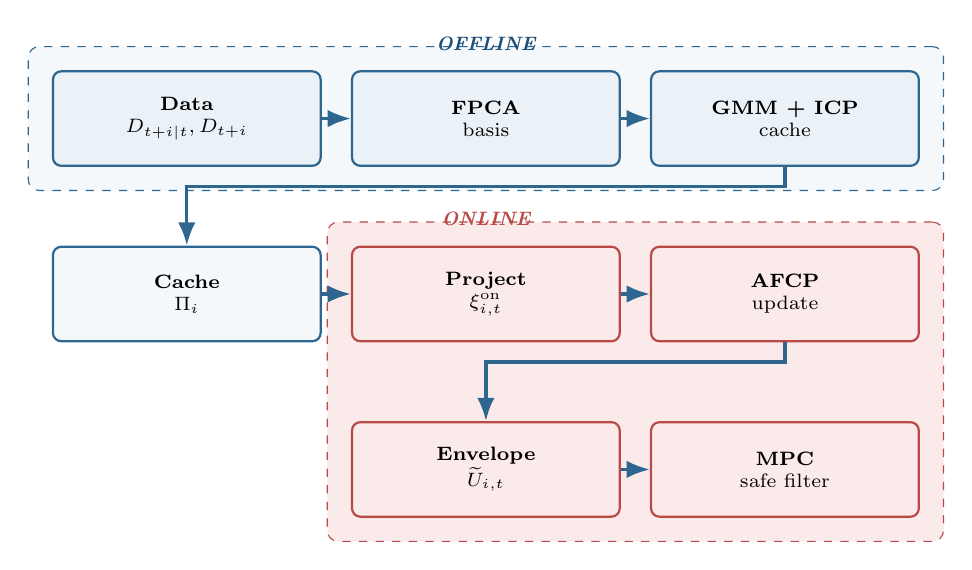
\begin{tikzpicture}[
    node distance=2.7mm and 3.7mm,
    every node/.style={font=\scriptsize},
    blockA/.style={rectangle,rounded corners=3pt,draw=snunavy2,thick,
      fill=snulight,align=center,minimum width=34mm,minimum height=12mm,inner sep=1.8pt},
    blockB/.style={rectangle,rounded corners=3pt,draw=accentred2,thick,
      fill=accentredlight,align=center,minimum width=34mm,minimum height=12mm,inner sep=1.8pt},
    arrow/.style={-Latex,very thick,snunavy2},
    label/.style={font=\scriptsize\itshape,text=textgray},
  ]
  \node[blockA] (cal) {\textbf{Data}\\$D_{t+i\mid t},D_{t+i}$};
  \node[blockA,right=of cal] (fpca) {\textbf{FPCA}\\basis};
  \node[blockA,right=of fpca] (gmm) {\textbf{GMM + ICP}\\cache};
  \node[label,above=1.3mm of fpca] {\textcolor{snunavy}{\bfseries OFFLINE}};
  \draw[arrow] (cal) -- (fpca);
  \draw[arrow] (fpca) -- (gmm);
  \node[blockA,below=10mm of cal,fill=snulight2] (cache) {\textbf{Cache}\\$\Pi_i$};
  \draw[arrow] (gmm.south) -- ++(0,-2.5mm) -| (cache.north);
  \node[blockB,right=of cache] (proj) {\textbf{Project}\\$\xi^{\mathrm{on}}_{i,t}$};
  \node[blockB,right=of proj] (afcp) {\textbf{AFCP}\\update};
  \draw[arrow] (cache) -- (proj);
  \draw[arrow] (proj) -- (afcp);
  \node[blockB,below=10mm of proj] (env) {\textbf{Envelope}\\$\widetilde U_{i,t}$};
  \node[blockB,right=of env] (mpc) {\textbf{MPC}\\safe filter};
  \draw[arrow] (afcp.south) -- ++(0,-2.5mm) -| (env.north);
  \draw[arrow] (env) -- (mpc);
  \node[label,above=1.3mm of proj] {\textcolor{accentred2}{\bfseries ONLINE}};
  \begin{pgfonlayer}{background}
    \node[fit=(cal)(gmm),fill=snulight2,rounded corners,inner sep=3mm,draw=snunavy2,dashed] {};
    \node[fit=(proj)(afcp)(env)(mpc),fill=accentredlight,rounded corners,inner sep=3mm,draw=accentred2,dashed] {};
  \end{pgfonlayer}
  \end{tikzpicture}}
  \caption{Overview of the proposed functional CP-informed MPC.
  \textbf{Offline} (blue): predicted and realized signed-distance fields are reduced by
  FPCA and a GMM-based inductive conformal procedure into a cached coefficient-envelope
  tuple $\Pi_i$.
  \textbf{Online} (red): the realized residual is projected onto the cached basis, the
  coefficient upper bound is adapted by the AFCP rule~\eqref{eq:acp_update}, and the
  resulting envelope $\widetilde U_{i,t}$ tightens the sampled-MPC safety filter.
  In the open 3D setting the online branch is unnecessary---ample free space makes the
  offline hard envelope sufficient---whereas the dense 2D benchmarks additionally exploit
  the online adaptation.}
  \label{fig:overview}
\end{figure}

\subsection{Mathematical Setup}

\subsubsection{Geometric property and tracking assumption.}
We first state the geometric regularity and tracking hypothesis used to transfer the conformal field bound into a robust safety constraint.

\begin{property}[Lipschitz continuity of the signed distance field]
\label{prop:sdf_lipschitz}
For any closed obstacle set $\mathcal O \subset \mathcal X$, the signed distance function $D(x,\mathcal{O})$
is $1$-Lipschitz on $\mathcal X$, i.e.,
\[
|D(x,\mathcal O)-D(y,\mathcal O)| \le \|x-y\|,
\qquad \forall x,y\in\mathcal X.
\]
\end{property}


% \begin{assumption}[Bounded tracking error]
% \label{ass:tracking_error}
% The low-level tracking controller follows the planned position $p^*_{t+i|t}$ with a uniform error bound $\epsilon > 0$:
% \[
% \|\mathbf{x}_{t+i}-\mathbf{x}^*_{t+i|t}\| \le \epsilon,
% \qquad \forall i\in\{1,\dots,N\}.
% \]
% \end{assumption}



% \subsubsection{Nominal predicted distance and conformal lower bound.}
% At planning time $t$, let $\widehat{\mathcal O}_{t+i|t}$ denote the predicted obstacle set at horizon step $i\in\{1,\dots,N\}$.
% The corresponding nominal signed-distance prediction is
% \begin{equation}
% D_{t+i|t}(x)
% \coloneqq
% d\!\left(x,\widehat{\mathcal O}_{t+i|t}\right)
% =
% \min_{o\in\widehat{\mathcal O}_{t+i|t}}\|x-o\|,
% \qquad x\in\mathcal X .
% \label{eq:D_nominal_mpc}
% \end{equation}
% Recall from \eqref{eq:functional-score} that the residual score field is
% \[
% S_{t+i|t}(x)=D_{t+i|t}(x)-D_{t+i}(x).
% \]
% The offline calibration procedure in Section~\ref{sec:gmm_ellipsoids} yields an initial upper envelope, which is then updated online through a coefficient-space adaptive rule.
% Accordingly, we define the online envelope at horizon index $i$ and planning time $t$ by $\widetilde U_{i,t}(x)$, and the corresponding conformalized lower-bound field by
% \begin{equation}
% \underline D_{t+i|t}(x)
% \coloneqq
% \max\!\left\{D_{t+i|t}(x)-\widetilde U_{i,t}(x),\,0\right\},
% \qquad x\in\mathcal X.
% \label{eq:lower_field_def}
% \end{equation}

\subsubsection{Robust CP-safe set via constraint tightening.}
Let
\[
r_{\mathrm{safe}} = r_{\mathrm{robot}} + r_{\mathrm{obs}}
\]
denote the nominal safety radius.
The conformal envelope $\widetilde U_{i,t}$ grows with the horizon index $i$ as prediction errors compound, so enforcing the full clearance $r_{\mathrm{safe}}$ against \emph{every} far-horizon step makes the conformal constraint increasingly conservative and can shrink the feasible set to the point of emptiness. To curb this long-horizon conservativeness---without weakening the near-term constraint that governs the control actually applied---we relax the required clearance with the time-to-go, following an inevitable-collision-state (ICS) argument~\cite{fraichard2004inevitable}: under bounded controls the robot retains the maneuverability to evade an obstacle that is still several steps away. Concretely, we introduce a horizon-dependent evasion budget
\begin{equation}
\Delta_i \coloneqq \tfrac{1}{2}\, a_{\mathrm{lat}}^{\max}\,\bigl((i-1)\Delta t\bigr)^2,
\qquad a_{\mathrm{lat}}^{\max} = v_{\max}\,\omega_{\max},
\label{eq:ics_budget}
\end{equation}
which lower-bounds the lateral displacement the controller can realize over the $i-1$ steps remaining before horizon index $i$.
Combining Property~\ref{prop:sdf_lipschitz}, Assumption~\ref{ass:tracking_error}, and the budget~\eqref{eq:ics_budget}, we define the robustly tightened, ICS-relaxed conformal safe set
\begin{equation}
\mathcal S^{\mathrm{cp}}_{t+i|t}
\coloneqq
\left\{x\in\mathcal X:\ \underline D_{t+i|t}(x)\ge \max\!\bigl(r_{\mathrm{safe}}+\epsilon-\Delta_i,\,0\bigr)\right\}
\label{eq:cp_safe_set_mpc}
\end{equation}
for $i=1,\dots,N$.
Because $\Delta_1=0$, the first (immediately applied) step retains the full tightened clearance $r_{\mathrm{safe}}+\epsilon$, and the relaxation loosens only the later, repeatedly re-planned steps.
Consequently the closed-loop guarantees of Theorems~\ref{thm:asymptotic_safety} and~\ref{thm:asymptotic_safety_afcp}, whose proofs invoke the constraint only at the applied $i=1$ step, continue to hold verbatim; the same effective radius $\max(r_{\mathrm{safe}}+\epsilon-\Delta_i,0)$ is reused inside the soft safety-shaping penalty.

\subsubsection{Sampled candidate trajectories.}
Rather than solving a nonlinear program exactly, we use a sampled MPC implementation.
At each planning step, we draw $K_p$ candidate input sequences
\[
\mathcal U_{\mathrm{cand}}
=
\{\mathbf u^{(1)},\dots,\mathbf u^{(K_p)}\},
\qquad
\mathbf u^{(k)}
=
\langle
u^{(k)}_{t|t},\dots,u^{(k)}_{t+N-1|t}
\rangle,
\]
where $u^{(k)}_{t+i|t}=(v^{(k)}_{t+i|t},\omega^{(k)}_{t+i|t})\in\mathcal U$ is sampled from
\[
\mathcal U=[v_{\min},v_{\max}]\times[\omega_{\min},\omega_{\max}].
\]

\subsubsection{Rollout and feasibility filtering.}
For each sampled plan $\mathbf u^{(k)}$, the predicted state trajectory is generated by forward simulation:
\begin{equation}
z^{(k)}_{t|t}=z_t,
\quad
z^{(k)}_{t+i+1|t}
=
f_r\!\left(z^{(k)}_{t+i|t},u^{(k)}_{t+i|t}\right),
\label{eq:rollout_sampled_mpc}
\end{equation}
for $i=0,\dots,N-1$.
Let $p^{(k)}_{t+i|t}\in\mathbb R^2$ denote the planar position corresponding to $z^{(k)}_{t+i|t}$.
A candidate trajectory is feasible if
\begin{equation}
p^{(k)}_{t+i|t}\in \mathcal S^{\mathrm{cp}}_{t+i|t},
\qquad \forall i\in\{1,\dots,N\}.
\label{eq:sampled_feasible_mpc}
\end{equation}

\subsubsection{Monte Carlo CP-MPC objective.}
Define the per-step margin by which a position falls short of the tightened, ICS-relaxed clearance,
\begin{equation}
g_{t+i|t}(x):=\max\!\bigl(r_{\mathrm{safe}}+\epsilon-\Delta_i,\,0\bigr)-\underline D_{t+i|t}(x),
\label{eq:soft_margin}
\end{equation}
so that the CP-safe set is the zero-sublevel set $\mathcal S^{\mathrm{cp}}_{t+i|t}=\{x:\,g_{t+i|t}(x)\le 0\}$.

Among the candidate trajectories, the planner selects the control sequence solving the finite-horizon problem
\begin{align}
\min_{k\in\{1,\dots,K_p\}}
\ \ &
\sum_{i=0}^{N-1}
\ell\!\left(z^{(k)}_{t+i|t},u^{(k)}_{t+i|t};p_{\mathrm{goal}}\right)
\nonumber\\
&\quad +
\ell_f\!\left(z^{(k)}_{t+N|t};p_{\mathrm{goal}}\right)
\label{eq:mc_cp_mpc_obj}
\\
\text{s.t.}\quad
&
z^{(k)}_{t+i+1|t}
=
f_r\!\left(z^{(k)}_{t+i|t},u^{(k)}_{t+i|t}\right),
\quad i=0,\dots,N-1, \nonumber\\
&
p^{(k)}_{t+i|t}\in \mathcal S^{\mathrm{cp}}_{t+i|t},
\quad i=1,\dots,N . \nonumber
\end{align}
This is the \emph{hard} formulation: it rejects outright any candidate that leaves $\mathcal S^{\mathrm{cp}}_{t+i|t}$ at some horizon step, and is the setting to which the guarantees of Theorems~\ref{thm:asymptotic_safety} and~\ref{thm:asymptotic_safety_afcp} apply. Alternatively, the dynamic constraint can be relaxed into a graded penalty, in the spirit of soft-constrained MPC~\cite{scokaert1999feasibility,kerrigan2000soft}. The planner then solves
\begin{align}
\min_{k\in\{1,\dots,K_p\}}
\ \ &
\sum_{i=0}^{N-1}
\ell\!\left(z^{(k)}_{t+i|t},u^{(k)}_{t+i|t};p_{\mathrm{goal}}\right)
+
\ell_f\!\left(z^{(k)}_{t+N|t};p_{\mathrm{goal}}\right)
\nonumber\\
&\quad +\,
w\sum_{i=1}^{N}\Bigl[\max\!\bigl(0,\,g_{t+i|t}(p^{(k)}_{t+i|t})\bigr)\Bigr]^2
\label{eq:soft_penalty}\\
\text{s.t.}\quad
&
z^{(k)}_{t+i+1|t}
=
f_r\!\left(z^{(k)}_{t+i|t},u^{(k)}_{t+i|t}\right),
\quad i=0,\dots,N-1, \nonumber
\end{align}
which retains only the dynamics constraint. The squared hinge charges only incursions into the calibrated unsafe region ($g_{t+i|t}>0$), discouraging---rather than forbidding---them. The weight $w>0$ is fixed rather than adapted, so~\eqref{eq:soft_penalty} is a quadratic-penalty relaxation~\cite{nocedal2006numerical} of the hard problem~\eqref{eq:mc_cp_mpc_obj}: its minimizer approaches the hard-constrained solution as $w\to\infty$. For finite $w$, it stays well-defined even where the hard feasible set is empty, at the cost of the strict closed-loop guarantee. We compare both formulations in our 2D pedestrian experiments.

\subsection{Notes on Computational Complexity}\label{subsec:complexity}




\subsection{Offline GMM Initialization}
\label{subsec:offline_online_cp}

\noindent
{\bf Dataset.} During the offline stage, we assume an access to $n_{\text{cal}}$ independent observations of length $T$:
\begin{equation*}
\left\{ \mathcal{O}^{(j)}_t : 0 \leq t \leq T,\; 1 \leq j \leq  n_{\text{cal}}  \right\}
\end{equation*}
from which we obtain the distance dataset for $i$-th planning step:
\begin{equation*}
\mathcal{D}_{\mathrm{cal},i} \coloneqq
\left\{S_{t+i|t}^{(j)}: 0\leq t \leq T - i, 1 \leq j \leq n_{\text{cal}} \right\}.
\end{equation*}
Then, we apply FPCA to obtain an orthonormal basis
\begin{equation*}
\{\varphi_{i,1},\dots,\varphi_{i,p_i}\},
\end{equation*}
This in turn produces the coefficient vector of each $S \in \mathcal{D}_{\text{cal}, i}$ according to~\eqref{eq:coefficient}.

The key design principle is to separate the field-level \emph{statistical initialization}, computed once offline, from the \emph{lightweight adaptation} performed online.
Offline, we exploit a large calibration dataset and a flexible GMM to construct the most accurate initial coefficient upper bound possible; this cost is paid only once, before deployment.
Online, the GMM is no longer evaluated---the controller adapts the cached upper bound directly from streaming residual observations and a prescribed target violation level, so the per-step cost stays small.

\paragraph{Time-to-go indexing.}
For each horizon index $i\in\{1,\dots,N\}$, we define the residual field
\begin{equation}
S_i(x)\equiv S_{t+i|t}(x)=D_{t+i|t}(x)-D_{t+i}(x),
\qquad x\in\mathcal X.
\label{eq:Si_def}
\end{equation}
We assume that the distribution of residual fields depends primarily on the time-to-go index $i$, which allows the offline initialization to be performed once per horizon step and reused online.

\paragraph{Offline calibration via FPCA and GMM.}
For each $i$, we collect a calibration dataset
\[
\mathcal D_{\mathrm{cal},i}
=
\{S_i^{(1)},\dots,S_i^{(n_{\mathrm{cal}})}\}.
\]
We then apply FPCA to obtain an orthonormal basis
\[
\{\varphi_{i,1},\dots,\varphi_{i,p_i}\},
\]
and represent each residual field by its coefficient vector
\begin{equation}
\xi_i(S)
=
\Bigl(
\langle S,\varphi_{i,1}\rangle,\dots,\langle S,\varphi_{i,p_i}\rangle
\Bigr)^\top
\in\mathbb R^{p_i}.
\label{eq:coeff_def_mpc}
\end{equation}
Using the coefficient dataset
$
\{\xi_i(S_i^{(j)})\}_{j=1}^{n_{\mathrm{cal}}},
$
we fit a Gaussian mixture model and apply the coefficient-space conformal construction of Section~\ref{sec:gmm_ellipsoids}.
This produces an accurate \emph{initial} coefficient upper bound
$
\hat{\xi}^{(0)}_i \in \mathbb R^{p_i}_{\ge 0},
$
together with the projection slack $\varepsilon_i$.
Equivalently, the initial offline envelope can be written as
\begin{equation}
U_i^{(0)}(x)
=
\varepsilon_i+\hat{\xi}^{(0)\top}_i \varphi_i(x),
\label{eq:Ui_init}
\end{equation}
where $\varphi_i(x)\in\mathbb R^{p_i}$ denotes the vector of basis evaluations at $x$.
The role of the offline GMM is therefore to provide the most accurate initialization $\hat{\xi}^{(0)}_i$ before deployment.

\paragraph{Cached offline tuple.}
For each horizon index $i$, we cache the offline calibration tuple
\begin{equation}
\Pi_i
\;\coloneqq\;
\Bigl(
\{\varphi_{i,m}\}_{m=1}^{p_i},\,
\hat{\xi}^{(0)}_i,\,
\varepsilon_i
\Bigr),
\label{eq:Pi_i_tuple}
\end{equation}
and denote by
\begin{equation}
\boldsymbol{\Pi}\coloneqq\{\Pi_i\}_{i=1}^N
\label{eq:Pi_collection}
\end{equation}
the full collection of horizon-indexed tuples cached by the controller.
Crucially, after deployment, the online controller uses only $\boldsymbol{\Pi}$ and no longer requires the fitted GMM itself.

\subsection{Online adaptive update}\label{subsec:online_update}
Once the robot starts moving, the GMM is used only for the initialization above and is not evaluated online.
At time $t$, if a realized residual field becomes available for horizon index $i$, we project it onto the cached basis:
\begin{equation}
\xi^{\mathrm{on}}_{i,t}
=
\Bigl(
\langle S^{\mathrm{on}}_{i,t},\varphi_{i,1}\rangle,\dots,
\langle S^{\mathrm{on}}_{i,t},\varphi_{i,p_i}\rangle
\Bigr)^\top .
\label{eq:online_coeff}
\end{equation}
As in the offline stage, this projection is evaluated on the discretization grid $\bar{\mathcal X}$ of Section~\ref{sec:score-comp}: it uses only the realized signed-distance residual at these grid points and costs $O(p_i |\bar{\mathcal X}|)$ per horizon index, so the full workspace field need not be reconstructed online.
We then compare the magnitude of each component of $\xi^{\mathrm{on}}_{i,t}$ against the current online upper bound
$\hat{\xi}^{(t)}_i$.
If the empirical violation frequency is above the target level $\alpha_{\mathrm{target}}$, the upper bound is inflated; if it is below the target level, the upper bound is contracted.
Hence the online update operates directly on the coefficient upper bound\cite{gibbs2021adaptiveconformalinferencedistribution},
\begin{equation}
\hat{\xi}_{i}^{(t+1)} = \hat{\xi}_{i}^{(t)} + \gamma \cdot \left( \mathbb{I}(|\xi_{i,t}^{\text{on}}| > \hat{\xi}_{i}^{(t)}) - \alpha_{\text{target}} \right).
\label{eq:acp_update}
\end{equation}
The corresponding online envelope is then
\begin{equation}
\widetilde U_{i,t}(x)
=
\varepsilon_i+\hat{\xi}^{(t)\top}_i \varphi_i(x).
\label{eq:Ui_online}
\end{equation}
Thus, offline GMM fitting is used only to initialize $\hat{\xi}^{(0)}_i$, while online adaptation operates entirely on the cached coefficients $\hat{\xi}^{(t)}_i$, without re-evaluating the GMM.

\paragraph{Optional grid realization for fast online evaluation.}
Although the primary cached objects are the tuples in~\eqref{eq:Pi_collection}, the envelope~\eqref{eq:Ui_online} may also be evaluated on a fixed workspace grid $\mathcal G$ and stored as a tensor for fast pointwise lookup.
This grid realization is purely an implementation-level acceleration.

\paragraph{Pointwise online evaluation along rollouts.}
For each candidate trajectory and each horizon step, the controller evaluates
\[
\underline D_{t+i|t}\!\left(p^{(k)}_{t+i|t}\right)
=
\max\!\left\{
D_{t+i|t}\!\left(p^{(k)}_{t+i|t}\right)
-
\widetilde U_{i,t}\!\left(p^{(k)}_{t+i|t}\right),
\,0
\right\},
\]
and accepts the trajectory only if the tightened safety condition~\eqref{eq:sampled_feasible_mpc} holds at every step.

\paragraph{Computational implications.}
This decomposition has two important consequences.
First, the computationally expensive statistical modeling is performed only once offline, where large-scale data and a flexible GMM can be used to obtain an accurate initialization.
Second, the online controller avoids all GMM computations and updates only the low-dimensional coefficient upper bound $\hat{\xi}^{(t)}_i$, which substantially reduces online overhead and better matches real-time operation.

Algorithm~\ref{alg:fcp_mpc_acp} summarizes the resulting procedure.

\begin{algorithm}[t]
\caption{Functional CP-informed MPC with offline GMM initialization and online coefficient-space adaptive update}
\label{alg:fcp_mpc_acp}
\begin{algorithmic}[1]
\STATE \textbf{Input:} Calibration dataset $\{\mathcal D_{\mathrm{cal},i}\}_{i=1}^N$, safety radius $r_{\mathrm{safe}}$, tracking margin $\epsilon$, target violation level $\alpha_{\mathrm{target}}$, workspace grid $\mathcal G$.
\STATE \textbf{Offline initialization:}
\FOR{each horizon index $i=1,\dots,N$}
    \STATE Compute residual-field samples $S_i^{(j)}(x)=D_{t+i|t}^{(j)}(x)-D_{t+i}^{(j)}(x)$;
    \STATE Apply FPCA and extract basis $\{\varphi_{i,m}\}_{m=1}^{p_i}$;
    \STATE Project all residual fields to obtain coefficient vectors $\xi_i^{(j)}$;
    \STATE Fit a GMM in coefficient space and compute the initial coefficient upper bound $\hat{\xi}^{(0)}_i$;
    \STATE Compute the projection slack $\varepsilon_i$;
    \STATE Cache the tuple $\Pi_i=(\{\varphi_{i,m}\}_{m=1}^{p_i},\hat{\xi}^{(0)}_i,\varepsilon_i)$;
\ENDFOR
\STATE Retain only the cached tuples $\{\Pi_i\}_{i=1}^N$; the GMM is not used online.
\STATE \textbf{Online MPC loop} (online adaptation optional):
\FOR{$t=0,1,2,\dots$}
    \STATE Observe current robot state $z_t$ and obtain obstacle predictions $\{\widehat{\mathcal O}_{t+i|t}\}_{i=1}^N$;
    \FOR{each horizon index $i$ for which an online residual field $S^{\mathrm{on}}_{i,t}$ becomes available}
        \STATE Project $S^{\mathrm{on}}_{i,t}$ onto the cached basis and compute $\xi^{\mathrm{on}}_{i,t}$;
        \STATE Update the coefficient upper bound $\hat{\xi}^{(t+1)}_i$ \eqref{eq:acp_update};

    \ENDFOR
    \STATE Sample candidate input sequences and roll out candidate trajectories;
    \STATE Evaluate $\widetilde U_{i,t}(x)=\varepsilon_i+\hat{\xi}^{(t)\top}_i\varphi_i(x)$ along rollouts;
    \STATE Filter infeasible trajectories using $\underline D_{t+i|t}(x)\ge r_{\mathrm{safe}}+\epsilon$;
    \STATE Select the feasible candidate minimizing~\eqref{eq:mc_cp_mpc_obj};
    \STATE Apply the first control input and advance to the next planning step;
\ENDFOR
\end{algorithmic}
\end{algorithm}

\section{Safety Analysis and Asymptotic Guarantees}

This section establishes the safety guarantees of the proposed framework.
A key advantage of the functional formulation is that pointwise safety holds for \emph{any} planned trajectory satisfying the tightened conformal constraint, independent of how the control space is sampled---precisely because the bound is certified over the entire field rather than along a single path.

We first present the base safety theorem, assuming the functional envelope covers the true score; we then extend it to a robust guarantee for dynamic environments through the online adaptive update.

\subsection{Base Safety Guarantee via Functional Coverage}

The following theorem demonstrates that if the spatial envelope asymptotically covers the true score function, the MPC framework guarantees the safety of the closed-loop system.

\begin{theorem}[Asymptotic Safety Guarantee]
\label{thm:asymptotic_safety}
Suppose that the Monte Carlo CP-MPC problem~\eqref{eq:mc_cp_mpc_obj} is feasible for all $t \ge 0$.
Let $p_{t+1}$ be the actual robot position at time $t+1$, and suppose the tracking error satisfies
\[
\|p_{t+1}-p^*_{t+1|t}\| \le \epsilon.
\]
Further suppose that the online envelope $\widetilde U_{1,t}$ satisfies the asymptotic coverage property
\[
\lim_{T\to\infty}\frac{1}{T}\sum_{t=0}^{T-1}
\mathbb I\!\left[
S_{t+1|t}(x)\le \widetilde U_{1,t}(x)\ \ \forall x\in\mathcal X
\right]
=
1-\alpha
\qquad \text{w.p. 1.}
\]
Then the closed-loop system is asymptotically $(1-\alpha)$-safe:
\begin{equation}
\liminf_{T \to \infty}
\frac{1}{T}\sum_{t=0}^{T-1}
\mathbb{I}\!\left[ D_{t+1}(p_{t+1}) \ge r_{\mathrm{safe}} \right]
\ge 1-\alpha,
\qquad \text{w.p. 1.}
\label{eq:asymptotic_safety_guarantee}
\end{equation}
\end{theorem}

\begin{proof}
For each $t$, define the event
\[
\mathcal E_{t+1}
\coloneqq
\left\{
S_{t+1|t}(x)\le \widetilde U_{1,t}(x)\ \ \forall x\in\mathcal X
\right\}.
\]
By construction of the lower-bound field in~\eqref{eq:lower_field_def}, on the event $\mathcal E_{t+1}$ we have
\[
D_{t+1}(x)\ge D_{t+1|t}(x)-\widetilde U_{1,t}(x)\ge \underline D_{t+1|t}(x),
\qquad \forall x\in\mathcal X.
\]

Since the MPC problem is feasible, the selected optimal plan satisfies the tightened safety constraint~\eqref{eq:sampled_feasible_mpc}. In particular,
\begin{equation}
\underline D_{t+1|t}(p^*_{t+1|t}) \ge r_{\mathrm{safe}}+\epsilon.
\label{eq:proof_feas_tight}
\end{equation}
Therefore, on $\mathcal E_{t+1}$,
\begin{equation}
D_{t+1}(p^*_{t+1|t})
\ge
\underline D_{t+1|t}(p^*_{t+1|t})
\ge
r_{\mathrm{safe}}+\epsilon.
\label{eq:proof_nominal_safe}
\end{equation}

Next, by Property~\ref{prop:sdf_lipschitz} and the tracking assumption,
\begin{equation}
\begin{aligned}
D_{t+1}(p_{t+1})
&\ge
D_{t+1}(p^*_{t+1|t})-\|p_{t+1}-p^*_{t+1|t}\| \\
&\ge
D_{t+1}(p^*_{t+1|t})-\epsilon.
\end{aligned}
\label{eq:proof_lipschitz}
\end{equation}
Combining \eqref{eq:proof_nominal_safe} and \eqref{eq:proof_lipschitz}, we obtain, on $\mathcal E_{t+1}$,
\[
D_{t+1}(p_{t+1}) \ge (r_{\mathrm{safe}}+\epsilon)-\epsilon = r_{\mathrm{safe}}.
\]
Hence,
\[
\mathbb I\!\left[D_{t+1}(p_{t+1})\ge r_{\mathrm{safe}}\right]
\ge
\mathbb I[\mathcal E_{t+1}].
\]
Averaging over $t=0,\dots,T-1$ and taking $\liminf$ yields
\[
\begin{aligned}
\liminf_{T\to\infty}
\frac{1}{T}\sum_{t=0}^{T-1}
\mathbb I\!\left[D_{t+1}(p_{t+1})\ge r_{\mathrm{safe}}\right]
&\ge
\lim_{T\to\infty}
\frac{1}{T}\sum_{t=0}^{T-1}\mathbb I[\mathcal E_{t+1}] \\
&=
1-\alpha
\end{aligned}
\]
with probability one, which proves~\eqref{eq:asymptotic_safety_guarantee}.
\end{proof}

\subsection{Robust Guarantee under Online Adaptation}

Theorem~\ref{thm:asymptotic_safety} establishes the foundational logic mapping functional coverage to pointwise safety. In offline calibration settings, guaranteeing the exact equality of the coverage (i.e., $\lim_{T\to\infty} \dots = 1-\alpha$) heavily relies on the exchangeability of the calibration and test data. However, in dynamic environments, unpredicted distribution shifts can invalidate this assumption.

To robustify our framework against such shifts, we drop the exchangeability assumption and employ the online Adaptive Functional Conformal Prediction (AFCP) method. By utilizing online learning and regret minimization in the coefficient space (as established in Section X.X), the AFCP update rule mathematically guarantees a robust lower bound on the functional coverage:
\begin{equation}
\liminf_{T\to\infty}\frac{1}{T}\sum_{t=0}^{T-1}
\mathbb I\!\left[
S_{t+1|t}(x)\le \widetilde U_{1,t}(x)\ \forall x\in\mathcal X
\right]
\ge
1-\alpha
\label{eq:afcp_coverage_prop}
\end{equation}
with probability one.

Based on this robust property, the following theorem extends the safety guarantee to dynamic, non-exchangeable environments.

\begin{theorem}[Asymptotic Safety with AFCP]
\label{thm:asymptotic_safety_afcp}
Consider a dynamic environment where data exchangeability does not hold. Suppose the feasibility and tracking conditions of Theorem~\ref{thm:asymptotic_safety} are satisfied. If the functional envelope $\widetilde U_{1,t}$ is updated online via the AFCP rule satisfying \eqref{eq:afcp_coverage_prop}, then the closed-loop system robustly maintains the asymptotic $(1-\alpha)$-safety:
\begin{equation}
\liminf_{T \to \infty}
\frac{1}{T}\sum_{t=0}^{T-1}
\mathbb{I}\!\left[ D_{t+1}(p_{t+1}) \ge r_{\mathrm{safe}} \right]
\ge 1-\alpha,
\qquad \text{w.p. 1.}
\end{equation}
\end{theorem}

\begin{proof}
Let $\mathcal E_{t+1} \coloneqq \{ S_{t+1|t}(x)\le \widetilde U_{1,t}(x)\ \forall x\in\mathcal X \}$ be the functional coverage event.
Following the exact same derivations as in the proof of Theorem~\ref{thm:asymptotic_safety}—specifically regarding the tightened MPC constraint \eqref{eq:proof_feas_tight} and the Lipschitz continuity of the SDF \eqref{eq:proof_lipschitz}—we establish that for any step $t$, the functional coverage directly implies point-wise safety:
$\mathbb I\!\left[D_{t+1}(p_{t+1})\ge r_{\mathrm{safe}}\right] \ge \mathbb I[\mathcal E_{t+1}]$.

Taking the average over $T$ steps and applying the limit infimum on both sides, we obtain:
\[
\liminf_{T\to\infty} \frac{1}{T}\sum_{t=0}^{T-1} \mathbb I\!\left[D_{t+1}(p_{t+1})\ge r_{\mathrm{safe}}\right] \ge \liminf_{T\to\infty} \frac{1}{T}\sum_{t=0}^{T-1}\mathbb I[\mathcal E_{t+1}].
\]
By substituting the AFCP coverage guarantee \eqref{eq:afcp_coverage_prop} into the right-hand side, we immediately conclude:
\[
\liminf_{T\to\infty} \frac{1}{T}\sum_{t=0}^{T-1} \mathbb I\!\left[D_{t+1}(p_{t+1})\ge r_{\mathrm{safe}}\right] \ge 1-\alpha.
\]
This completes the proof, verifying that the point-wise safety of the robot is inherently guaranteed by the online adaptation of the functional envelope.
\end{proof}


\section{Experimental Setup}
We evaluate the proposed \emph{Conformal SDF} framework and its integration into a model predictive controller.
Our experiments are designed to assess how functional conformal calibration of
the signed distance field affects safety, feasibility, and efficiency in
closed-loop motion planning under prediction uncertainty.

To this end, we conduct experiments at increasing levels of complexity:
a 2D toy setting for visualizing conformalized distance fields,
standard 2D pedestrian navigation benchmarks for quantitative evaluation, and
a challenging 3D quadrotor navigation task for assessing closed-loop performance
under dense, uncertain dynamics.

Across all settings, conformal prediction is applied to calibrate a lower bound
of the predicted signed distance field, which is then enforced as a hard safety
constraint within MPC.

\paragraph{CP Calibration}
We collect a calibration dataset of length $T_{\mathrm{cal}}$ and compute
residual SDF fields $R_{t+i\mid t}(x) = D_{t+i\mid t}(x) - D_{t+i}(x)$ over a
3D grid for each horizon step $i \in \{1,\dots,H\}$.
The residual fields are projected onto a $p$-dimensional subspace using PCA and
modeled via a $K$-component Gaussian mixture model (GMM) in coefficient space.
We set the target miscoverage level to $\alpha$ and compute horizon-dependent
upper envelopes $U_{t+i\mid t}(x)$, yielding the conformal lower-bound SDF
defined in~\eqref{eq:lower_field_def}.

\subsection{Conformal SDF Visualization at 2D}
Figure~\ref{fig:sdf_visualization_2d} shows an illustrative 2D example where the
conformal lower bound expands the unsafe region in areas of high uncertainty.


\begin{figure}[t]
    \centering
    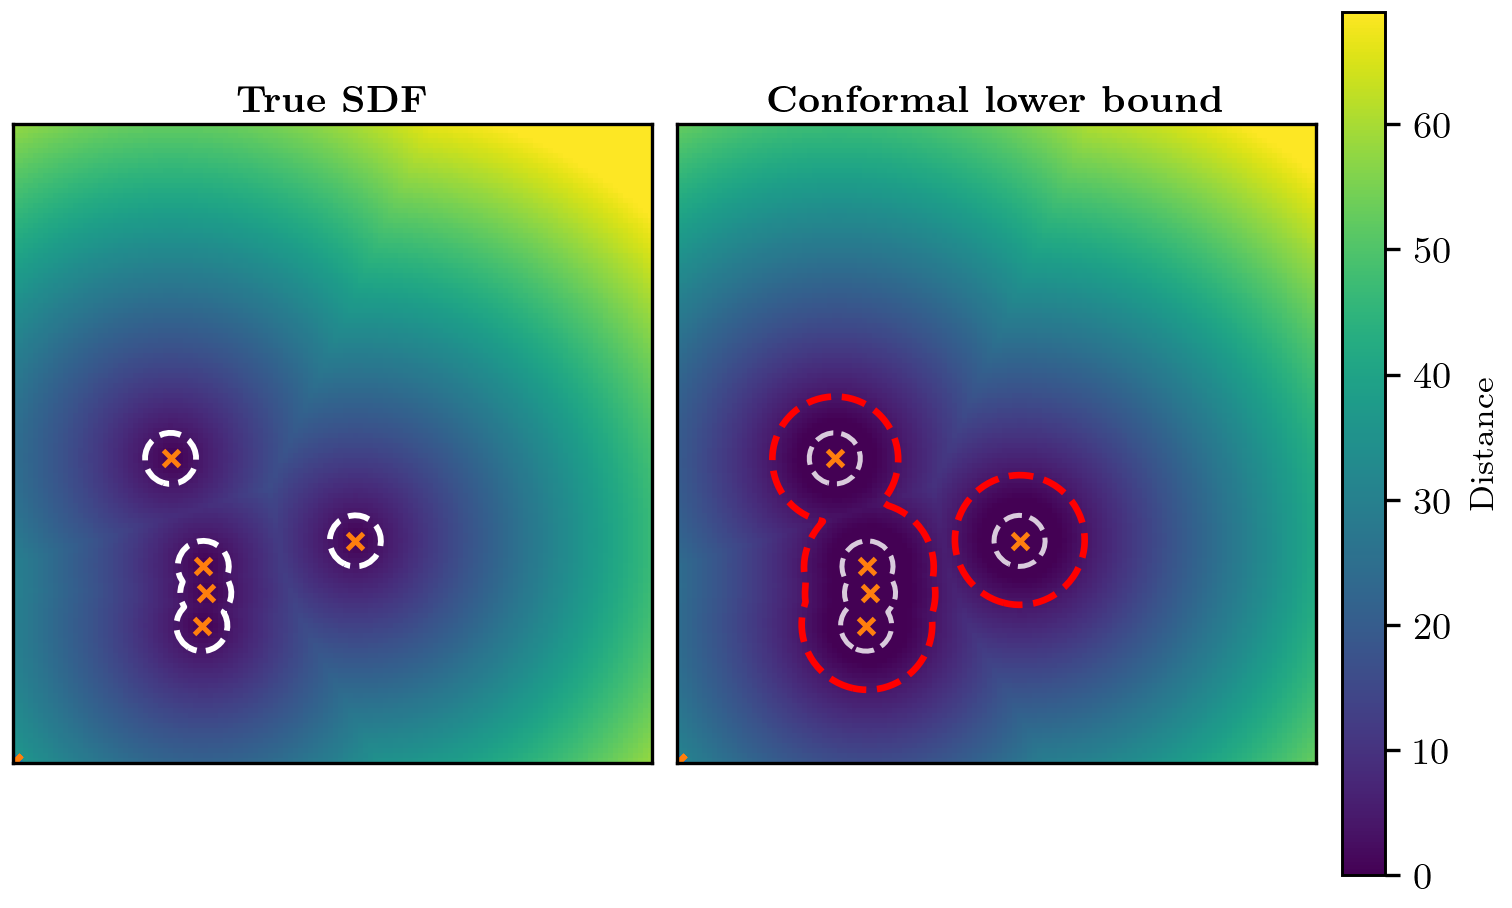
\includegraphics[width=\columnwidth]{multi_obs_H2.png}
    \caption{2D conformal SDF visualization at a representative time.
    \textbf{Left:} ground-truth signed distance field.
    \textbf{Right:} conformal lower-bound field.
    Dashed contours indicate the safety threshold $r_{\mathrm{safe}}$.}
    \label{fig:sdf_visualization_2d}
\end{figure}

\subsection{CP-Informed MPC in 2D Pedestrian Environments}

Before evaluating the proposed framework in complex 3D scenarios, we first
validate its effectiveness in standard 2D pedestrian navigation benchmarks.
These experiments serve as a controlled testbed to examine how spatial
conformal calibration affects safety, feasibility, and efficiency in a
well-studied setting.

\paragraph{2D Simulation Setup}
We evaluate all methods on all five ETH--UCY pedestrian datasets---
\texttt{eth}, \texttt{hotel}, \texttt{univ}, \texttt{zara1}, and \texttt{zara2}.
Pedestrian trajectories are taken from real-world recordings, and a mobile robot
is tasked with navigating toward a fixed goal while avoiding dynamic pedestrians.

At each planning step, the robot observes recent pedestrian state histories and
receives predicted future trajectories over a fixed planning horizon.
A Trajectron++~\cite{salzmann2020trajectron}
predictor is used as the base prediction model.
This setup allows us to isolate the effect of \emph{offline error calibration}
independently of the prediction model itself.

\subsubsection{Robot dynamics.}
Let the robot state be $z_t=(x_t,y_t,\theta_t)\in\mathbb R^2\times S^1$ and the control input be
$u_t=(v_t,\omega_t)\in\mathcal U$.
We use the discrete-time unicycle model
\[
z_{t+1}=f_r(z_t,u_t)
=
\begin{bmatrix}
x_t+\Delta t\,v_t\cos\theta_t\\
y_t+\Delta t\,v_t\sin\theta_t\\
\theta_t+\Delta t\,\omega_t
\end{bmatrix}.
\]

The robot is modeled as a unicycle system with bounded linear and angular velocities.
For a fair comparison, all methods share the same trajectory sampler, planning
horizon, and cost structure, including goal-tracking and control-effort terms.

We compare four controllers spanning how prediction uncertainty is handled:
\begin{itemize}
\item \emph{CC-MPC}: safety through soft penalty terms, without explicit uncertainty calibration;
\item \emph{ECP-MPC}: explicit online reasoning about prediction uncertainty;
\item \emph{ACP-MPC}: online adaptation of conformal bounds; and
\item \emph{FCP-MPC} (ours): offline functional conformal calibration of the signed-distance field.
\end{itemize}
For FCP-MPC we evaluate both a hard- and a soft-constraint formulation, ablating in
each case the online coefficient adaptation of~\eqref{eq:acp_update} to assess its
effect on overconservatism at long horizons.



\paragraph{Evaluation Metrics}
We report four closed-loop metrics (lower is better), averaged over the scenes of
each dataset:
\begin{itemize}
\item \emph{collision rate}: fraction of planning steps that violate the safety threshold;
\item \emph{infeasible rate}: fraction of steps for which no feasible trajectory is found;
\item \emph{time-to-goal}: number of planning steps to reach the goal; and
\item \emph{control time}: average per-step computation (ms).
\end{itemize}


\paragraph{Hard vs.\ soft use of the conformal bound in 2D}
In the 2D pedestrian benchmarks, we evaluate two variants of FCP-MPC that differ
in how the conformal lower-bound signed distance field is incorporated.

\emph{Hard-CP} enforces the conformal bound strictly as a hard feasibility
constraint over the entire planning horizon.
In dense 2D scenes, the offline functional envelope can become overly conservative
as the horizon increases due to compounding prediction errors, which significantly
shrinks the feasible set and leads to a high infeasible rate.

\emph{Soft-CP} instead incorporates the conformal lower bound only as a soft
safety-shaping penalty in the MPC objective: it keeps a hard feasibility filter for
static obstacles but not for the predicted dynamic obstacles, ranking candidates by
their conformal safety margin.
Because the dynamic conformal bound no longer constrains the feasible set, the planner
rarely exhausts its feasible candidates, trading the worst-case feasibility guarantee
for consistently low infeasibility and shorter paths.
Table~\ref{tab:2d_results} reports the main comparison against the baselines, while
Table~\ref{tab:2d_ablation} isolates the effect of the online envelope adaptation
within each variant.


\subsection{CP-Informed MPC in 3D}
We embed the conformal SDF into MPC by replacing the nominal distance constraint
with the conformal lower bound:
\begin{equation}
\underline{D}_{t+i\mid t}(x_{t+i}) \ge r_{\mathrm{safe}}, \qquad i=1,\dots,H.
\end{equation}

\paragraph{3D Experimental Setup}
We evaluate FCP-MPC in a challenging physics-based quadrotor navigation task
implemented in PyBullet.
The robot is modeled as a quadrotor with a low-level PID controller running at
240\,Hz, while the high-level MPC planner operates at a slower planning period
$\Delta t = 0.1\,\mathrm{s}$.

The environment contains $M = 280$ dynamic obstacles, modeled as kinematic agents
with stochastic mode switching among multiple motion patterns, including
constant-velocity, turning, wandering, and stop-and-go behaviors.
Additive process noise is applied to obstacle dynamics, inducing increasing
prediction uncertainty over the planning horizon.
Obstacles are rendered as spheres within a bounded 3D workspace
$x,y \in [-3,7]$, $z \in [0,8]$.

At each planning step the controller receives recent obstacle state histories and
predicted obstacle trajectories over a horizon $H = 12$; oracle future trajectories
are provided solely for evaluation and metric computation.
A constant-velocity predictor is used as the base prediction model, and prediction
noise is injected to emulate model mismatch.

Due to the higher-dimensional workspace and the availability of sufficient
free space in 3D, we employ a \emph{fully offline} functional conformal
calibration in this setting.
Unlike the 2D case, excessive conservativeness does not immediately block
progress, allowing the calibrated worst-case safety envelopes to be enforced
directly without additional online adaptation.

The planner samples endpoint candidates and generates smooth quintic polynomial
trajectories in $\mathbb{R}^3$.
Unsafe trajectories are filtered using the conformal lower-bound SDF constraint,
and the minimum-cost feasible trajectory is selected.
Each episode terminates once the robot reaches the goal within
$0.25\,\mathrm{m}$ or a maximum step limit is reached.


\paragraph{Evaluation Metrics}
We use the same closed-loop metrics as in the 2D study---collision rate, infeasible
rate, time-to-goal, and per-step runtime---with collision now defined by the minimum
robot--obstacle distance violating $r_{\mathrm{safe}}$. For spatial evaluation we
additionally report the \emph{containment} of the unsafe set (whether the true unsafe
region lies inside the conformal unsafe region) and a voxel-wise \emph{recall} of the
true unsafe set. All metrics are averaged over the evaluated scenes of each dataset.



\section{Results and Analysis}
Qualitative rollouts indicate that FCP-MPC adapts conservativeness to spatially
varying uncertainty: it becomes more conservative in crowded or uncertain regions
while remaining less restrictive in open areas.

\subsection{2D Pedestrian Navigation}
Table~\ref{tab:2d_results} reports quantitative results on the ETH--UCY pedestrian
datasets, and Figure~\ref{fig:traj_2d} shows representative closed-loop trajectories
of FCP-MPC and the baselines.
Several consistent trends emerge across all environments.

CC-MPC exhibits consistently zero infeasible rates due to its soft safety
penalty formulation.
However, this robustness comes at the cost of conservative behavior, leading to
slow progress toward the goal and frequent timeouts in complex scenes such as
\texttt{univ}.
Moreover, while collisions are reduced compared to nominal planning, they remain
non-negligible in dense pedestrian scenarios, indicating limited ability to
anticipate worst-case interactions.

ECP-MPC achieves strong nominal safety, often attaining among the lowest collision
rates and the shortest steps-to-goal when successful.
Nevertheless, its explicit online reasoning over uncertainty incurs substantial
computational overhead.
In all datasets, the control computation time exceeds tens of milliseconds and
approaches or surpasses the planning period, which leads to degraded closed-loop
performance, increased infeasible rates, and occasional failures to reach the
goal.

ACP-MPC reduces computational cost by simplifying uncertainty handling and
achieves fast control updates.
However, the online adaptation of conformal bounds remains insufficient to
robustly handle dense and highly dynamic environments, resulting in elevated
infeasible rates and frequent timeouts despite relatively low collision rates in
some datasets.

FCP-MPC reveals a clear safety--efficiency trade-off between its hard and soft
variants.
The hard variant enforces the conformal lower bound as a strict feasibility
constraint, attaining the lowest collision rates (e.g., $0.023$ on \texttt{eth})
but a non-zero infeasible rate, since the worst-case envelope can become
overconservative at long horizons.
The soft variant instead enforces the bound only as a penalty, eliminating
infeasibility across all datasets and substantially reducing steps-to-goal
relative to CC-MPC, at the cost of a higher collision rate in the densest scenes
(e.g., \texttt{zara2}, \texttt{univ}).
Importantly, both variants keep the control computation time far below ECP-MPC---often
by close to an order of magnitude---because uncertainty calibration is performed
offline and only a low-dimensional coefficient update runs online.
Together, the two variants show that the same offline-calibrated field supports both a
strict feasibility constraint and a soft safety penalty, trading conservativeness for
feasibility as the scene demands.

Overall, these results demonstrate that offline functional conformal calibration
enables FCP-MPC to reason over global uncertainty distributions without expensive
online computation.
By decoupling uncertainty calibration from real-time control, FCP-MPC achieves a
favorable balance between safety, feasibility, and efficiency in crowded dynamic
environments.

\begin{table*}[!t]
\centering
\small
\caption{2D navigation results on ETH--UCY pedestrian datasets.
All metrics are averaged across scenes; lower is better.
The FCP-MPC (hard) and FCP-MPC (soft) rows use our full method with the
\emph{online-adapted} (AFCP) envelope of~\eqref{eq:acp_update};
Table~\ref{tab:2d_ablation} ablates the fixed offline (FCP) versus
online-adapted (AFCP) choice for each constraint mode.}
\label{tab:2d_results}
\begin{tabular}{llcccc}
\hline
Dataset & Method & Collision rate $\downarrow$ & Infeasible rate $\downarrow$ & Steps to goal $\downarrow$ & Ctrl.\ time (ms) $\downarrow$ \\
\hline
eth & ACP-MPC~\cite{dixit2023adaptive} & 0.062 & 0.223 & 71.7 & \textbf{0.61} \\
 & CC-MPC~\cite{lekeufack2024decision} & 0.055 & \textbf{0.000} & 99.0 & 0.66 \\
 & ECP-MPC~\cite{shin2025egocentric} & 0.042 & 0.226 & 62.0 & 34.91 \\
 & FCP-MPC (hard) & \textbf{0.023} & 0.265 & 73.7 & 2.56 \\
 & FCP-MPC (soft) & 0.165 & \textbf{0.000} & \textbf{34.0} & 3.11 \\
\hline
hotel & ACP-MPC~\cite{dixit2023adaptive} & \textbf{0.000} & 0.223 & 73.7 & \textbf{0.81} \\
 & CC-MPC~\cite{lekeufack2024decision} & 0.055 & \textbf{0.000} & timeout & 0.89 \\
 & ECP-MPC~\cite{shin2025egocentric} & \textbf{0.000} & 0.069 & 68.3 & 44.91 \\
 & FCP-MPC (hard) & 0.103 & 0.114 & 42.3 & 3.55 \\
 & FCP-MPC (soft) & 0.089 & \textbf{0.000} & \textbf{29.0} & 3.61 \\
\hline
univ & ACP-MPC~\cite{dixit2023adaptive} & \textbf{0.011} & 0.344 & timeout & \textbf{2.78} \\
 & CC-MPC~\cite{lekeufack2024decision} & 0.077 & \textbf{0.000} & timeout & 3.43 \\
 & ECP-MPC~\cite{shin2025egocentric} & 0.351 & 0.629 & 263.0 & 62.63 \\
 & FCP-MPC (hard) & 0.253 & 0.383 & timeout & 7.57 \\
 & FCP-MPC (soft) & 0.284 & \textbf{0.000} & \textbf{95.0} & 12.75 \\
\hline
zara1 & ACP-MPC~\cite{dixit2023adaptive} & 0.135 & 0.491 & 91.3 & \textbf{0.62} \\
 & CC-MPC~\cite{lekeufack2024decision} & 0.076 & \textbf{0.000} & 91.0 & 0.68 \\
 & ECP-MPC~\cite{shin2025egocentric} & \textbf{0.063} & 0.136 & 58.7 & 41.95 \\
 & FCP-MPC (hard) & 0.163 & 0.262 & 70.3 & 2.30 \\
 & FCP-MPC (soft) & 0.146 & \textbf{0.000} & \textbf{32.0} & 3.09 \\
\hline
zara2 & ACP-MPC~\cite{dixit2023adaptive} & 0.247 & 0.672 & 93.3 & \textbf{0.74} \\
 & CC-MPC~\cite{lekeufack2024decision} & \textbf{0.064} & \textbf{0.000} & 97.3 & 0.82 \\
 & ECP-MPC~\cite{shin2025egocentric} & 0.201 & 0.322 & 81.7 & 45.92 \\
 & FCP-MPC (hard) & 0.185 & 0.248 & 84.3 & 2.63 \\
 & FCP-MPC (soft) & 0.272 & \textbf{0.000} & \textbf{61.7} & 3.92 \\
\hline
\end{tabular}
\end{table*}

\begin{table*}[!t]
\centering
\footnotesize
\setlength{\tabcolsep}{4pt}
\caption{Ablation of the online envelope adaptation~\eqref{eq:acp_update} in 2D.
Within each constraint mode (Hard / Soft), the better value per metric is in bold.
Lower values indicate better performance.}
\label{tab:2d_ablation}
\begin{tabular}{lllcccc}
\hline
Dataset & Constraint & Online adapt. & Collision rate $\downarrow$ & Infeasible rate $\downarrow$ & Steps to goal $\downarrow$ & Ctrl.\ time (ms) $\downarrow$ \\
\hline
eth & Hard & No & 0.032 & 0.480 & \textbf{73.3} & \textbf{1.18} \\
 & Hard & Yes & \textbf{0.023} & \textbf{0.265} & 73.7 & 2.59 \\
 & Soft & No & 0.184 & N/A & 36.7 & \textbf{2.39} \\
 & Soft & Yes & \textbf{0.165} & N/A & \textbf{34.0} & 3.31 \\
\hline
hotel & Hard & No & 0.188 & 0.293 & 68.0 & \textbf{2.00} \\
 & Hard & Yes & \textbf{0.103} & \textbf{0.114} & \textbf{42.3} & 3.25 \\
 & Soft & No & \textbf{0.081} & N/A & 30.7 & \textbf{2.72} \\
 & Soft & Yes & 0.089 & N/A & \textbf{29.0} & 3.64 \\
\hline
univ & Hard & No & 0.393 & 0.640 & timeout & \textbf{2.69} \\
 & Hard & Yes & \textbf{0.253} & \textbf{0.383} & timeout & 7.65 \\
 & Soft & No & 0.299 & N/A & 97.0 & \textbf{9.27} \\
 & Soft & Yes & \textbf{0.284} & N/A & \textbf{95.0} & 12.71 \\
\hline
zara1 & Hard & No & 0.223 & 0.454 & 75.0 & \textbf{1.14} \\
 & Hard & Yes & \textbf{0.163} & \textbf{0.262} & \textbf{70.3} & 2.42 \\
 & Soft & No & \textbf{0.137} & N/A & 34.3 & \textbf{2.49} \\
 & Soft & Yes & 0.146 & N/A & \textbf{32.0} & 3.59 \\
\hline
zara2 & Hard & No & \textbf{0.169} & \textbf{0.241} & 88.7 & \textbf{1.79} \\
 & Hard & Yes & 0.185 & 0.248 & \textbf{84.3} & 2.74 \\
 & Soft & No & 0.303 & N/A & 62.7 & \textbf{2.84} \\
 & Soft & Yes & \textbf{0.272} & N/A & \textbf{61.7} & 4.06 \\
\hline
\end{tabular}
\end{table*}

\begin{figure*}[!t]
  \centering
  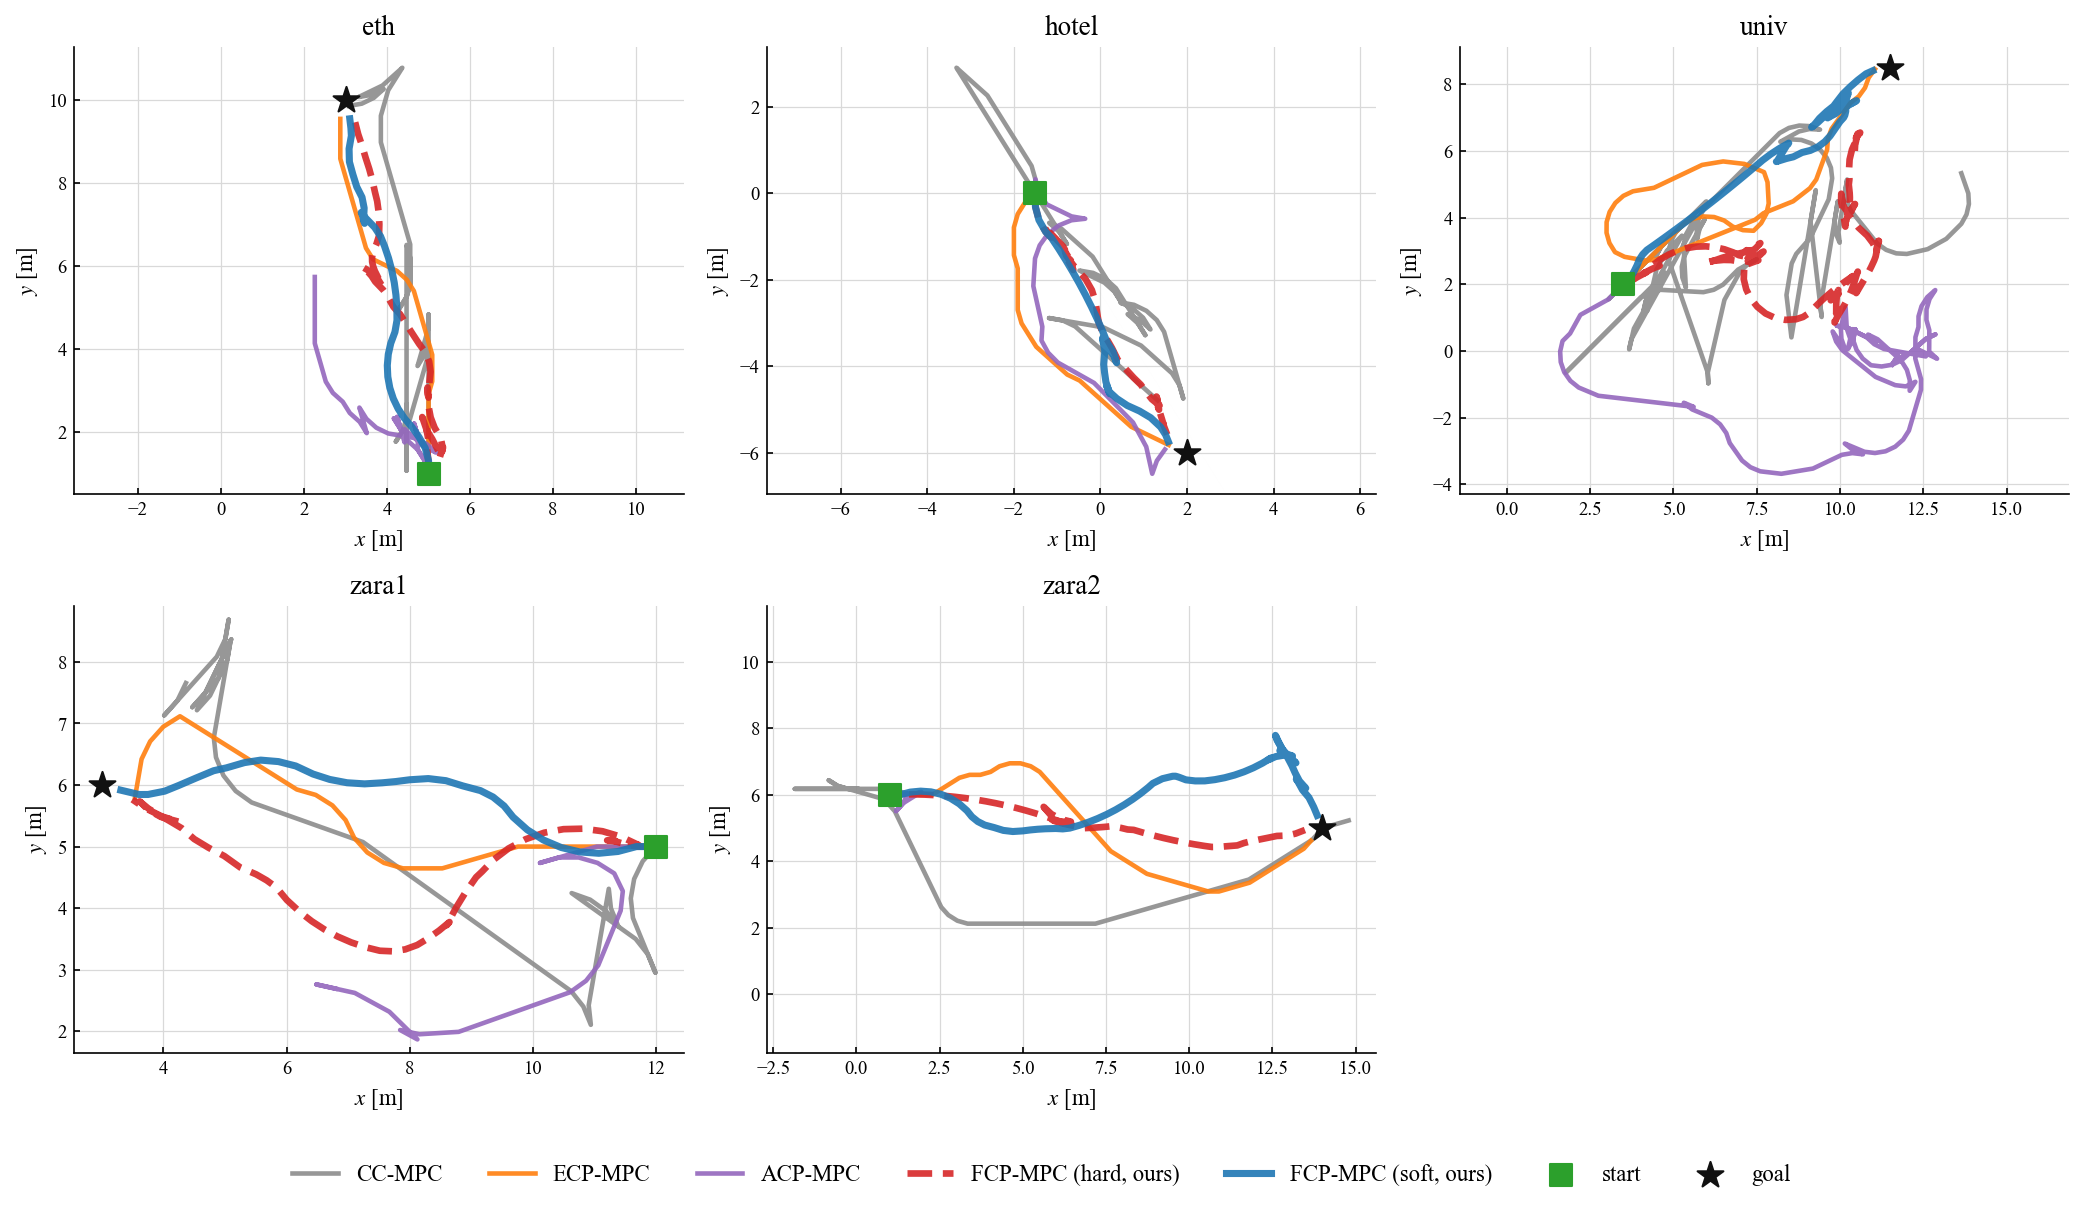
\includegraphics[width=\linewidth]{traj_2d.png}
  \caption{Representative closed-loop trajectories on one scene of each of the five
  ETH--UCY datasets (green squares: start; black stars: goal).
  Both variants of FCP-MPC (ours)---soft (thick blue) and hard (thick red)---reach
  the goal along direct paths, whereas the baselines, drawn in lighter lines, tend to
  wander or stall: CC-MPC (gray) is slow and conservative, ECP-MPC (orange) detours, and
  ACP-MPC (purple) often fails to make steady progress in dense scenes such as
  \texttt{univ}.}
  \label{fig:traj_2d}
\end{figure*}




\paragraph{Effect of online envelope adaptation}

The offline functional envelope is calibrated on held-out data and can become
overly conservative under the distribution shift of dense, dynamic scenes,
occasionally eliminating all feasible trajectories after hard filtering.
The online update~\eqref{eq:acp_update} addresses this by adapting the coefficient
upper bound $\hat{\xi}^{(t)}_i$ directly from realized residuals, without
re-invoking the GMM.
Table~\ref{tab:2d_ablation} isolates this effect.
For the hard variant, online adaptation markedly reduces the infeasible
rate---from $0.480$ to $0.265$ on \texttt{eth}, from $0.640$ to $0.383$ on
\texttt{univ}, and from $0.454$ to $0.262$ on \texttt{zara1}---by relaxing the
envelope where the offline bound was unnecessarily tight, while leaving collision
rates essentially unchanged.
For the soft variant, which is already feasible by construction, adaptation yields
only marginal changes.
Because the update operates on the low-dimensional coefficients evaluated on the
discretization grid of Section~\ref{sec:score-comp}, it adds only a few milliseconds
of online computation and stays well below the cost of ECP-MPC.

\begin{figure}[!t]
  \centering
  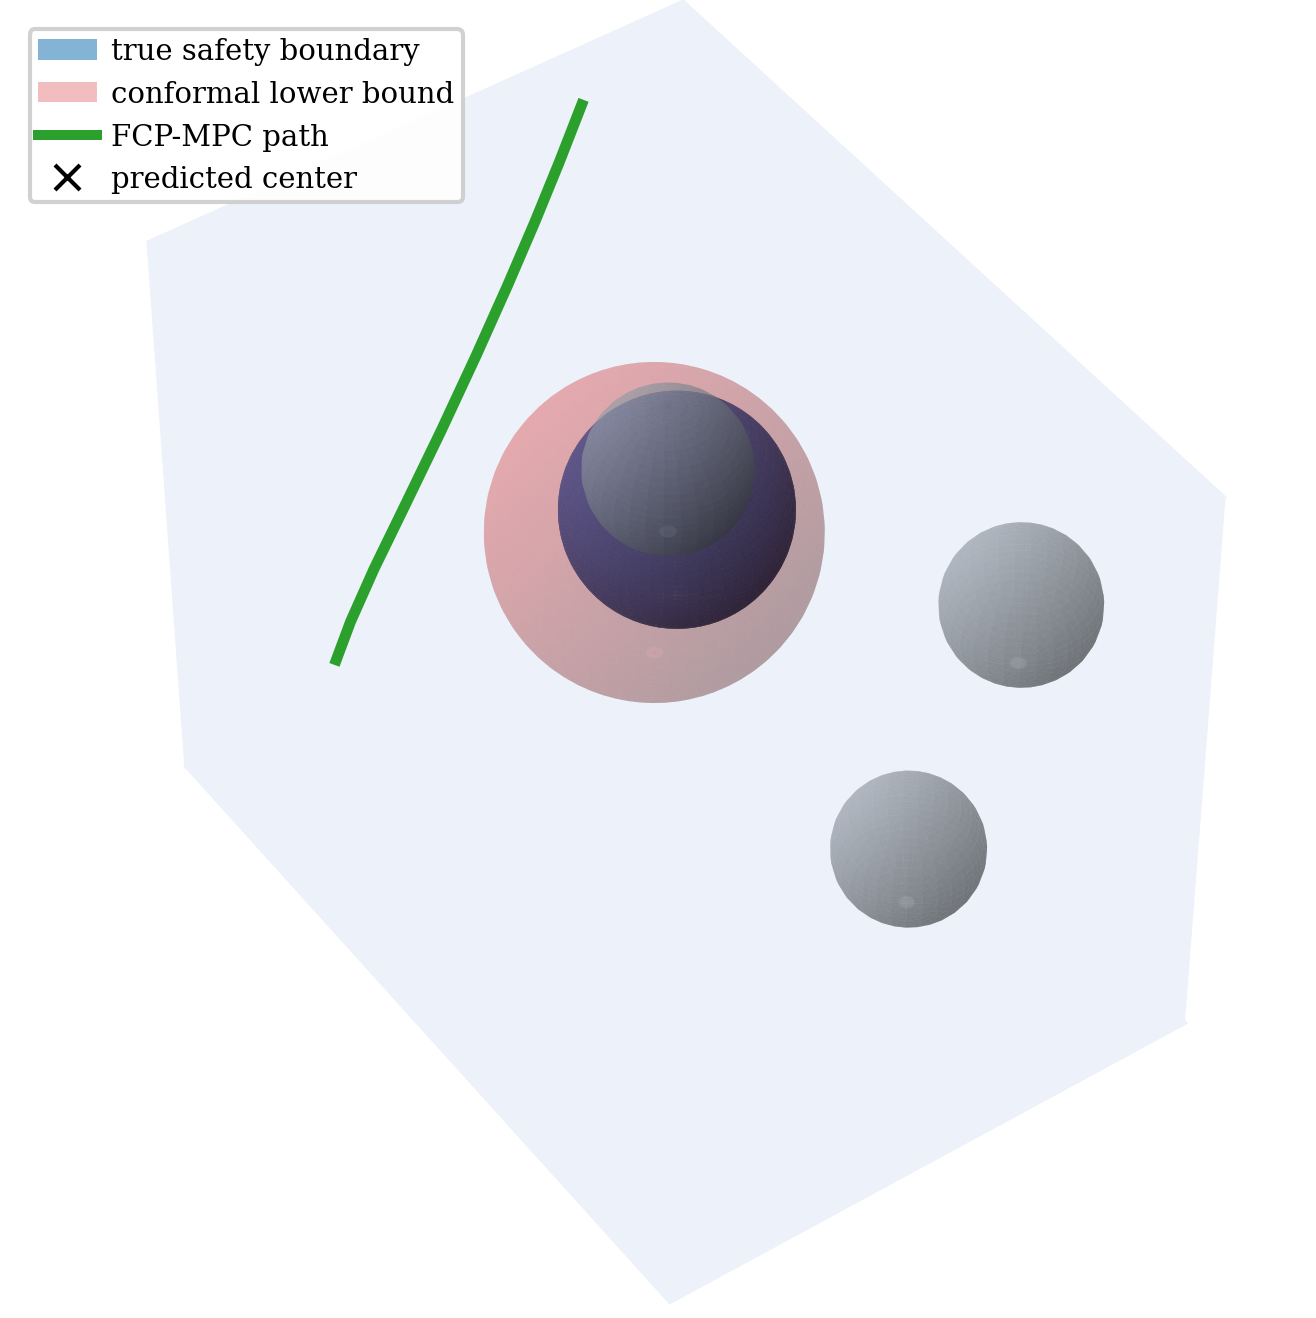
\includegraphics[width=\columnwidth]{Func_cp_3d_zoom.png}
  \caption{True and conformal safety bounds in 3D, zoomed onto a single obstacle.
  The solid blue ball is the \emph{true} safety boundary
  $D_{t+i}(x)=r_{\mathrm{safe}}$ around the actual obstacle (used only for
  evaluation); the translucent red shell is the \emph{conformal lower-bound}
  boundary $\underline{D}_{t+i\mid t}(x)=r_{\mathrm{safe}}$ obtained from the
  functional calibration, i.e.\ the nominal safety region around the predicted
  center inflated by the calibrated margin. The conformal surface
  encloses the true one, certifying coverage, and the executed FCP-MPC path
  (green) threads just outside it---progressing efficiently while respecting the
  worst-case safety constraint. Faint gray spheres are other obstacles in the
  scene.}
  \label{fig:fcp_3d}
\end{figure}



\subsection{3D Quadrotor Navigation}
Table~\ref{tab:pybullet_results} reports averaged closed-loop results in a
challenging scenario with $M=280$ dynamic obstacles and noisy
predictions (prediction noise $0.20$, obstacle process noise $0.22$, oracle
future noise $0.20$), evaluated over $17$ random seeds.

ACP-MPC~\cite{dixit2023adaptive} adapts a scalar conformal radius online via ACI,
but this pointwise-inflation approach becomes overly conservative in the dense 3D
workspace: the inflated spheres collectively block the sampled paths, so the planner is
frequently infeasible and the robot stalls and crashes within the first few steps, never
reaching the goal.
Its scalar calibration covers only single-horizon prediction errors, so the
aggregated obstacle inflation in 3D is too large to be useful.

CC-MPC exhibits a zero infeasible rate by construction due to its purely soft
safety formulation. It also incurs a low collision rate while
this conservative penalty-based strategy substantially slows progress toward
the goal, resulting in an increased time-to-goal that exceeds the
$250$-step time budget (timeout) in all seeds.


ECP-MPC is dominated by its online cost. Its exhaustive, per-step conformal evaluation
drives the control time to nearly one second per planning step ($977$~ms at
$M{=}280$; Fig.~\ref{fig:scalability_3d})---roughly an order of magnitude beyond the
real-time budget. The quadrotor therefore loses control authority almost immediately and
crashes within a handful of steps (about $16$ on average); its zero collision count merely
reflects that it never traverses the field.

FCP-MPC is the only method that reaches the goal in this dense regime, and its two
deployments of the \emph{same} offline-calibrated field expose a clear density effect.
Enforced as a \emph{hard} feasibility filter, FCP-MPC~(hard) inherits the formal guarantee
of Theorems~\ref{thm:asymptotic_safety}--\ref{thm:asymptotic_safety_afcp}; at this extreme
density, however, the worst-case envelope is conservative enough that the planner often has
no feasible candidate and stalls (infeasible rate $0.361$), so it reaches only $71\%$ of
seeds and, while stalled, is occasionally struck by a moving obstacle (collision $0.070$).
Enforced as a \emph{soft} penalty on the same field, FCP-MPC~(soft) never stalls (infeasible
rate $0.000$): it reaches the goal in \emph{every} seed at the lowest collision rate of any
method that traverses the field ($0.015$, well within the target $\alpha=0.10$), and runs in
real time at $80$~ms per step---an order of magnitude below ECP-MPC.
The same calibrated field thus supports both a certified hard constraint and a robust soft
penalty; in this densest regime the soft deployment is the better practical choice.
Table~\ref{tab:results_sparse} repeats the comparison at a lower obstacle count
($N_{\mathrm{obs}}=50$), so the methods are evaluated across a range of densities; we discuss
how the hard/soft trade-off shifts with density in Section~\ref{sec:discussion}.
Figure~\ref{fig:fcp_3d} illustrates the underlying conformal bound in 3D, and
Figure~\ref{fig:traj_3d} compares the closed-loop trajectories of CC-MPC, ECP-MPC, ACP-MPC,
and FCP-MPC~(soft) across three random seeds (panels~(a)--(c)) in the same
$M{=}280$-obstacle environment: FCP-MPC threads to the goal in every panel while the
baselines stall or fall (marked by a red~$\times$) early in the field.

\begin{figure*}[!t]
  \centering
  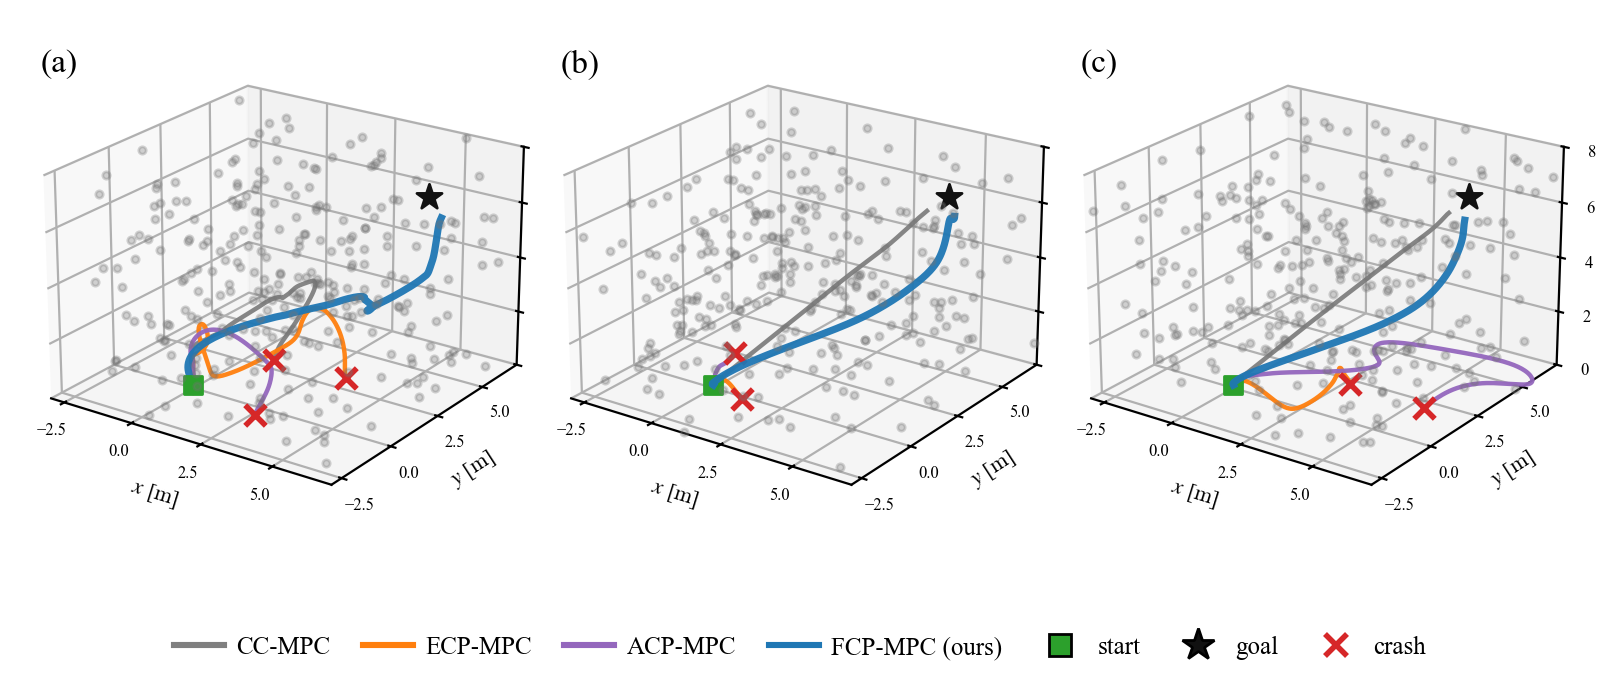
\includegraphics[width=\linewidth]{traj_3d_seeds.png}
  \caption{Closed-loop trajectory comparison in the dense 3D quadrotor task
  ($M{=}280$ dynamic obstacles) across three random seeds, shown in
  panels~(a)--(c). Each panel overlays all four controllers---CC-MPC (gray),
  ECP-MPC (orange), ACP-MPC (purple), and FCP-MPC (ours, blue). Green square:
  start; black star: goal; a red~$\times$ marks where a controller lost control
  and fell to the floor. FCP-MPC is the only method that makes consistent
  progress to the goal across seeds, while the baselines stall or crash early in
  the dense field.}
  \label{fig:traj_3d}
\end{figure*}

\begin{figure}[!t]
  \centering
  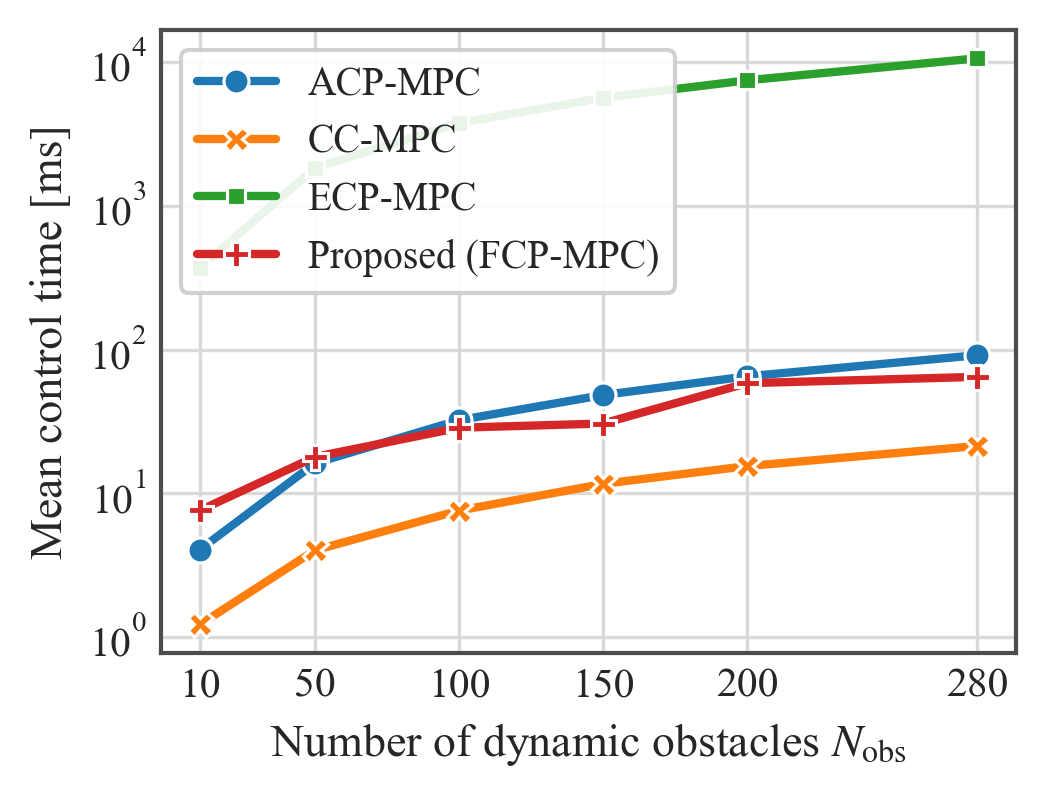
\includegraphics[width=\columnwidth]{control_time_3d.png}
  \caption{Scalability comparison of MPC methods in dense 3D environments.
  The figure reports the mean control computation time per planning step as a
  function of the number of dynamic obstacles.}
  \label{fig:scalability_3d}
\end{figure}


\begin{table*}[!t]
\centering
\small
\caption{3D quadrotor navigation results with $280$ dynamic obstacles, averaged over
$17$ seeds ($\alpha=0.10$). FCP-MPC~(hard) and FCP-MPC~(soft) deploy the \emph{same}
offline-calibrated field as a hard feasibility filter and as a soft penalty, respectively.
Steps-to-goal is averaged over successful episodes; ``crashed'' / ``timeout'' mark methods
that never reach the goal.}
\label{tab:pybullet_results}
\begin{tabular}{lcccc}
\hline
Method &
Collision rate $\downarrow$ &
Infeasible rate $\downarrow$ &
Steps to goal $\downarrow$ &
Ctrl.\ time (ms) $\downarrow$ \\
\hline
ACP-MPC~\cite{dixit2023adaptive}
& 0.032
& \textbf{0.130}
& crashed
& 216.9 \\
CC-MPC~\cite{lekeufack2024decision}
& 0.064
& N/A
& 186.5
& 215.3 \\
ECP-MPC~\cite{shin2025egocentric}
& 0.090
& 0.342
& crashed
& 306.4 \\
FCP-MPC (hard)
& 0.044
& 0.269
& 123.9
& \textbf{51.5} \\
FCP-MPC (soft)
& \textbf{0.032}
& N/A
& \textbf{84.8}
& 159.9 \\
\hline
\end{tabular}

\end{table*}

\begin{table*}[!t]
\centering
\small
\caption{3D quadrotor navigation at a lower obstacle count ($N_{\mathrm{obs}}=50$),
averaged over $17$ seeds ($\alpha=0.10$); same setup and columns as
Table~\ref{tab:pybullet_results}. Reporting both densities shows how each method behaves
as the workspace becomes less cluttered.}
\label{tab:results_sparse}
\begin{tabular}{lcccc}
\hline
Method &
Collision rate $\downarrow$ &
Infeasible rate $\downarrow$ &
Steps to goal $\downarrow$ &
Ctrl.\ time (ms) $\downarrow$ \\
\hline
ACP-MPC~\cite{dixit2023adaptive}
& 0.008
& \textbf{0.002}
& crashed
& 42.2 \\
CC-MPC~\cite{lekeufack2024decision}
& 0.019
& N/A
& 183.6
& 40.8 \\
ECP-MPC~\cite{shin2025egocentric}
& 0.059
& 0.107
& crashed
& 198.8 \\
FCP-MPC (hard)
& \textbf{0.012}
& 0.094
& 87.8
& \textbf{25.9} \\
FCP-MPC (soft)
& 0.015
& N/A
& \textbf{74.4}
& 38.2 \\
\hline
\end{tabular}

\end{table*}

\paragraph{Scalability Analysis in Dense 3D Environments}
To assess computational scalability, we compare the average planning-time
runtime of ACP-MPC, CC-MPC, ECP-MPC, and the proposed FCP-MPC as the number of
dynamic obstacles increases.
Figure~\ref{fig:scalability_3d} reports the mean control time per planning step
under increasingly dense 3D environments, with the number of obstacles ranging
from $N_{\mathrm{obs}} = 10$ to $280$.

ECP-MPC is one to two orders of magnitude slower than every other method at all
densities (hundreds to thousands of milliseconds per step versus tens of
milliseconds), reflecting the need for repeated pointwise conformal evaluations and
online aggregation of safety constraints across obstacles and horizon steps; it never
meets the real-time budget.
In contrast, FCP-MPC scales gracefully, maintaining
near-linear growth in computation time (from $7$~ms at $N_{\mathrm{obs}}=10$ to
$32$~ms at $N_{\mathrm{obs}}=280$) despite the high-dimensional workspace
and dense obstacle configuration.
This improvement stems from the fully offline functional calibration, which
allows safety evaluation to be reduced to efficient fieldwise SDF queries at
runtime.

CC-MPC remains the cheapest---it performs no uncertainty calibration---but offers
no probabilistic guarantee and incurs elevated collision rates in dense scenarios
(Table~\ref{tab:pybullet_results}). The scalar-radius ACP-MPC scales comparably to
FCP-MPC, yet it conformalizes only a single pointwise radius rather than the full
spatial field; FCP-MPC thus matches the inexpensive baselines in per-step cost
while retaining a calibrated safety \emph{field}.
Overall, the results demonstrate that FCP-MPC achieves a practical balance
between safety and computational efficiency, remaining real-time feasible even
in highly cluttered 3D environments with hundreds of dynamic obstacles.





\subsection{Discussion}
\label{sec:discussion}
\paragraph{Enforcing the calibrated bound in 2D.}
The 2D benchmarks isolate how the conformal lower bound should be \emph{used}
once it has been calibrated.
The hard variant attains the lowest collision rates but, because the worst-case
envelope compounds over the horizon, can become overconservative and leave a
non-zero infeasible rate; the soft variant removes this infeasibility by treating
the bound as a penalty rather than a hard constraint, at the price of a higher
collision rate in the densest scenes (Table~\ref{tab:2d_results}).
The online coefficient adaptation of~\eqref{eq:acp_update} directly counteracts the
overconservatism of the hard variant, substantially lowering its infeasible rate
while leaving collisions essentially unchanged (Table~\ref{tab:2d_ablation}).
Both effects reuse the offline calibration, so the added online cost is only a few
milliseconds---far below the tens of milliseconds required by ECP-MPC's explicit
online uncertainty reasoning.
These pedestrian experiments thus stress-test the fieldwise calibration in a regime
where free space is scarce, complementing the open 3D study below.



\paragraph{Separating calibration from real-time planning in 3D.}
The contrasting behaviors in Table~\ref{tab:pybullet_results} follow directly from
how each controller injects uncertainty and safety into the MPC formulation.

CC-MPC enforces safety through soft constraints embedded in a mixed cost
function.
This formulation allows the controller to locally maneuver around obstacles
rather than strictly avoiding worst-case configurations, which can be effective
in moderately cluttered scenes.
However, the reliance on soft penalties induces conservative trade-offs between
goal progress and safety, often prioritizing risk reduction over forward motion.
As a result, CC-MPC tends to exhibit slower trajectories and significantly
increased time-to-goal, despite eliminating infeasible planning steps.

ECP-MPC explicitly reasons about the surrounding environment and achieves the
lowest collision rates among all methods.
Nevertheless, this strong situational awareness comes at the cost of excessive
online computation.
Accounting for detailed, step-wise uncertainty during planning leads to control
latency that exceeds real-time limits, causing timeouts and
control-time-induced crashes.
This highlights a critical limitation: accurately modeling all contingencies
online can undermine closed-loop feasibility, even when nominal safety is
achieved.

FCP-MPC represents a deliberate trade-off between these two extremes.
Rather than reasoning about all uncertainty online, it leverages offline
functional conformal prediction to account for the full distribution of
uncertainty in a global and principled manner, so that at runtime safety reduces to a
fieldwise query against the cached bound, enabling efficient and predictable planning.

A practical advantage of the functional formulation is that this single offline-calibrated
field can be \emph{deployed} in different ways without recomputation: enforced as a hard
feasibility filter it yields the formal coverage guarantee, while enforced as a soft penalty
it shapes the planner's cost. Which is preferable is environment-dependent. In the dense 2D
pedestrian scenes, free space is scarce and the hard variant's worst-case envelope can
remove all feasible motions, so the soft variant (and the online adaptation) recover
feasibility. The open 3D workspace is less cluttered overall, yet at the highest obstacle count its fast,
maneuvering obstacles still make the hard envelope conservative enough to stall the planner
(infeasible rate $0.361$, reaching only $71\%$ of seeds at $N_{\mathrm{obs}}=280$;
Table~\ref{tab:pybullet_results}), whereas the soft deployment of the \emph{same} field
eliminates stalling and reaches every seed. This gap is density-dependent: as the obstacle
count is reduced to $N_{\mathrm{obs}}=50$ the hard variant is no longer overconservative and
again reaches reliably with a low collision rate (Table~\ref{tab:results_sparse}), confirming
that its stalling is specific to the densest, most dynamic regime. Across regimes, then, the
soft penalty is the more robust practical choice---especially in dense dynamic scenes---while
the hard filter is preferable wherever the workspace is open enough to keep it feasible and a
strict per-step guarantee is desired.

Crucially, this safety comes from the conformal field itself: FCP-MPC~(soft) keeps its
collision rate well within the target miscoverage level $\alpha = 0.10$ \emph{even as it
actively traverses} the dense field---consistent with the intended calibration behavior of
the conformal lower-bound SDF---whereas the baselines attain low collision counts only by
never traversing it. And it does so at $80$~ms per planning step---real-time, and an order
of magnitude faster than ECP-MPC's explicit online uncertainty reasoning.

The use of worst-case conformal bounds inevitably introduces conservativeness,
which leads to a non-zero infeasible rate when enforced as a hard constraint.
In contrast, CC-MPC employs purely soft safety penalties and therefore
exhibits near-zero infeasibility by construction.
However, because uncertainty calibration in FCP-MPC is performed offline,
the resulting online computation remains efficient, yielding a favorable
balance between safety, feasibility, and real-time performance.

Importantly, FCP-MPC~(soft) reaches the goal \emph{reliably}---in every seed, versus
partial or no success for the other methods---which we attribute to the spatially coherent
nature of the functional conformal calibration.
While point-wise or trajectory-wise calibration methods tend to induce locally
conservative behavior due to worst-case reasoning at individual states or
timesteps, the calibrated signed distance field provides a global view of
where safety margins are tight and where sufficient free space exists.
This allows the controller to commit to globally safe corridors and make steady progress,
rather than hesitating or stalling at local bottlenecks while still
respecting the calibrated safety constraint.

Overall, the results suggest that separating uncertainty modeling from online
planning, and calibrating uncertainty at the level of the spatial field rather
than individual points, is key to achieving reliable safety--performance
trade-offs in dense 3D navigation.

\section{Conclusion}

We presented FCP-MPC, a functional conformal prediction framework that calibrates
a high-confidence lower bound of the predicted signed distance field and enforces
it as a tightened safety constraint within a sampling-based model predictive
controller. By calibrating uncertainty at the level of the spatial \emph{field}---
rather than at individual states or trajectories---the method reasons about safety
globally and coherently, and its offline--online decomposition keeps the per-step
computation low: a GMM-based envelope is fitted offline, while online only a
low-dimensional coefficient vector is refined by a lightweight adaptive update. We
established asymptotic closed-loop safety both under exchangeability and, through
the online adaptation, under distribution shift.

Across the ETH--UCY pedestrian benchmarks and a dense 3D quadrotor task with up to
$280$ moving obstacles, FCP-MPC attained a favorable balance of safety,
feasibility, and efficiency, scaling far more gracefully than online
uncertainty-reasoning baselines while remaining real-time feasible.

\noindent
{\bf Limitations and future work.}
Because the calibrated envelope bounds the worst case, the hard-constrained variant
remains conservative and can still report a non-zero infeasible rate in the densest
2D scenes; the soft and online-adapted variants mitigate, but do not eliminate, this
trade-off. Our guarantees further assume a bounded low-level tracking error and a
\emph{fixed} functional basis. Relaxing these assumptions---learning the basis
online, folding perception and state-estimation error into the same conformal
pipeline, and extending the fieldwise calibration to richer robot and obstacle
dynamics---are promising directions, as are tighter integration with full-stack
perception and validation on physical hardware.


{\appendices

\section*{Derivation of $\breve{\mathsf{U}}_{t+i|t}$}\label{app:derivation}
\paragraph{Exact union-of-ellipsoids representation.{\color{teal} (will be moved to appendix)}}
Because $g$ is a maximum over mixture components,
$\mathscr{T}_{t+i\mid t}$ decomposes exactly as a union of component-wise ellipsoids
(cf.\ Eq.\ (9) in \cite{lei2015conformal}):
\begin{equation}
\begin{aligned}
\mathscr{T}_{t+i\mid t} &= \bigcup_{k=1}^K \mathscr{T}^{(k)}_{t+i\mid t}, \\
\mathscr{T}^{(k)}_{t+i\mid t} &\coloneqq \left\{\xi:\ \varphi(\xi;\widehat\mu_k,\widehat\Sigma_k)\ge \tfrac{\lambda_i}{\widehat\pi_k}\right\}.
\end{aligned}
\label{eq:exact_union}
\end{equation}
Each $\mathscr{T}^{(k)}_{t+i\mid t}$ is an ellipsoid
\begin{equation}
\mathscr{T}^{(k)}_{t+i\mid t}
=
\left\{\xi:\ (\xi-\widehat\mu_k)^\top \widehat\Sigma_k^{-1}(\xi-\widehat\mu_k)\le r_{k,i}^2\right\},
\label{eq:ellipsoid_def}
\end{equation}
where the radius is
\begin{equation*}
r_{k,i}^2
=
\max\!\left\{
0,\,
-2\log\!\left(
\frac{\lambda_i}{\widehat\pi_k}\,(2\pi)^{p_i/2}\sqrt{\det(\widehat\Sigma_k)}
\right)
\right\}.
\end{equation*}


\paragraph{From coefficient regions to a functional upper envelope}
\label{sec:upper_envelope}

Let the discretized basis vector at coordinate $x$ be
$\varphi_i(x)\in\mathbb{R}^{p_i}$ (in code, $\varphi_i(\cdot)$ is represented implicitly
by the PCA components $\phi_i$ over the discretized domain).
For coefficients $\xi\in\mathbb{R}^{p_i}$, the projected value is $\xi^\top \varphi_i(x)$.
Using~\eqref{eq:exact_union}, we finally define the upper bound $\breve{\mathsf{U}}_{t+i|t}(\mathbf{x})$ as
\begin{equation*}
\breve{\mathsf{U}}_{t+i|t}(\mathbf{x}) \coloneqq \sup_{\xi\in\mathscr{T}_{t+i\mid t}} \xi^\top \varphi_i(\mathbf{x})
=
\max_{1\le k\le K}\ \sup_{\xi\in\mathscr{T}^{(k)}_{t+i\mid t}} \xi^\top \varphi_i(\mathbf{x}).
\end{equation*}
For an ellipsoid~\eqref{eq:ellipsoid_def}, the inner supremum  is given in closed form:
\begin{equation}
\sup_{\xi\in\mathscr{T}^{(k)}_{t+i\mid t}} \xi^\top \varphi_i(\mathbf{x})
=
\widehat\mu_k^\top \varphi_i(\mathbf{x})
+
r_{k,i}\left(\varphi_i(\mathbf{x})^\top \widehat\Sigma_k\, \varphi_i(\mathbf{x})\right)^{1/2}.
\label{eq:ellipsoid_support_function}
\end{equation}

In implementation, we add a small diagonal jitter to $\widehat\Sigma_k$
for numerical stability.



}

\bibliographystyle{IEEEtran}
\bibliography{reference}

\end{document}
